% Chapter Template
\chapter{!!NOT DONE!! The CMS experiment at the LHC !!NOT DONE!!} \label{Chapter2} 



This chapter outlines the main characteristics of the Large
Hadron Collider (LHC) in Section~\ref{lhc} and of the Compact Muon Solenoid (CMS)
detector in Section~\ref{cms}. In Section~\ref{sec:reconstruction}, it is
given an explanation of the reconstruction algorithm, called
\emph{Particle flow}, and reconstruction performances are
discussed. The main focus of Sections~\ref{cms}
and~\ref{sec:reconstruction} will be on lepton (electrons and muons) identification and
reconstruction in consideration of the multilepton final states which are
discussed in Chapter~\ref{Chapter5} and~\ref{Chapter6} and thus are
central to this dissertation.



%----------------------------------------------------------------------------------------
%	SECTION 1
%----------------------------------------------------------------------------------------
\section{The Large Hadron Collider}\label{lhc}

The LHC~\cite{Brning2004LHCDR} is a circular particle accelerator
located at the CERN laboratories in Geneva operating since 10
September 2008. It is
designed to accelerate hadrons (like protons, Lead-ions, Xenon-ions) and to
operate at the centre-of-mass energy of 14\TeV.
The circular ring is installed in a tunnel of a 27 kilometers where
the Large Electron Positron collider~\cite{Lep:designReport} was
previously located.\\
A graphic representation of CERN accelerator
complex is shown in Figure~\ref{fig:cern} where the particle
accelerations begins at the LINAC, foregoing booster, PS and SPS, in
order. The LHC consists of accelerating components as well as
superconducting magnets to focus the hadrons, keep them on the right
trajectory and squeeze them tight together right before the
collision point. 

\begin{figure}[h]
\centering
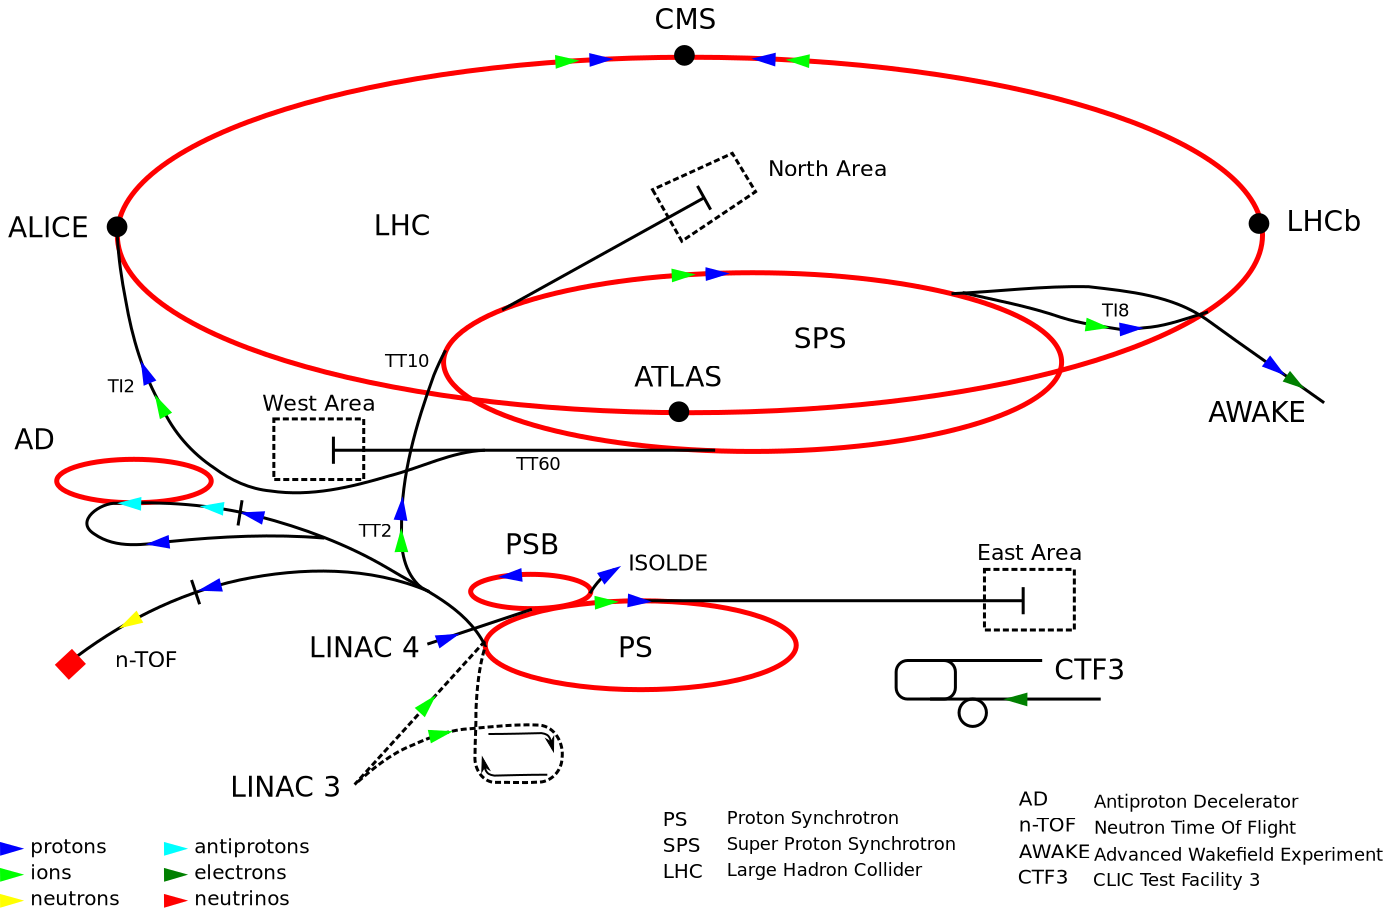
\includegraphics[width=0.75\textwidth]{Figures/c2/Cern-accelerator-complex.png}
\vspace*{3mm}
\caption{The LHC is the largest ring (top) in a complex chain of particle accelerators. The smaller machines are used in a chain to help boost the particles to their final energies and provide beams to a whole set of smaller experiments, which also aim to uncover the mysteries of the Universe~\cite{Mobs:2197559}}
\label{fig:cern}
\end{figure}

The protons are accelerated in opposite directions in two distinct
accelerator tubes which cross at four interactions points where the
protons are made to collide. At each of the interaction points along the ring,
four experiments are located with the aim to reconstruct the
sub-atomic particles which are made at the moment of a high energy
collision. The protons are grouped in bunches which are
accelerated in steps using the full accelerator chain consisting in a linear
accelerator, boosters, synchrotrons and, at the end, they are injected
into the LHC with an energy of 540\GeV where a system of
superconducting magnets further accelerate them up to 13\TeV. Every
25 ns collisions between proton bunches occur meaning 40 million
bunch crossing per second. At full regime during data taking time
period about 2800 bunches travel in the LHC rings and each bunch is
made of up to $1.1\times10^{11}$ protons.

The four experiments located at the four interaction points are
ALICE~\cite{alice_2008} (A Large Ion Collider Experiment),
ATLAS~\cite{atlas_2008} (A Toroidal LHC ApparatuS),
CMS~\cite{cms_2008} and LHCb~\cite{lhcb_2008} (Large Hadron Collider
beauty), refer to Figure~\ref{fig:cern}. ALICE experiment is designed
to study the presence and the properties of the hypothetical
quark-gluon plasma formed during heavy ions collisions, LHCb is
designed to be very sensitive in analyzing the properties of the B
mesons. The last two, ATLAS and CMS are general purpose detectors
designed to investigate a vast range of physics scenarios starting
from the search and discovery of the Higgs boson to extra dimensions
and dark matter. \\

The accelerator-dependent features and parameters which are important for a
physics analysis are the instantaneous and integrated luminosity, the
number, in the same bunch crossing, of simultaneous collisions and the
center-of-mass energy of the proton-proton collisions.

The instantaneous luminosity is defined as a time dependent
parameter, $d\mathcal{L}/dt$, which correlates the number of collisions
($N$) in a certain amount of time ($t$) and the cross section of a
given process through the relation:
\begin{equation}
\label{eq:instalumi}
\frac{dN}{dt} \: = \: \frac{d\mathcal{L}}{dt}\sigma
\end{equation}

The unit of the instantaneous luminosity is $b^{-1}s^{-1}$, where 1
barn $= 10^{-24} \ cm^2$ and it depends on the number of bunches in
the proton beam, on the number of protons per bunch and on the beam
optics. \\
The integrated luminosity is the integral of the instantaneous
luminosity over time, and relates the cross section of a
given process to the number of events $N$ of that process:
\begin{equation}
\label{eq:intelumi}
\mathcal{L} \:=\: \int \frac{d\mathcal{L}}{dt} dt \: = \: \frac{N}{\sigma}
\end{equation}


\begin{figure}[h]
  \noindent
  \makebox[\textwidth]{
  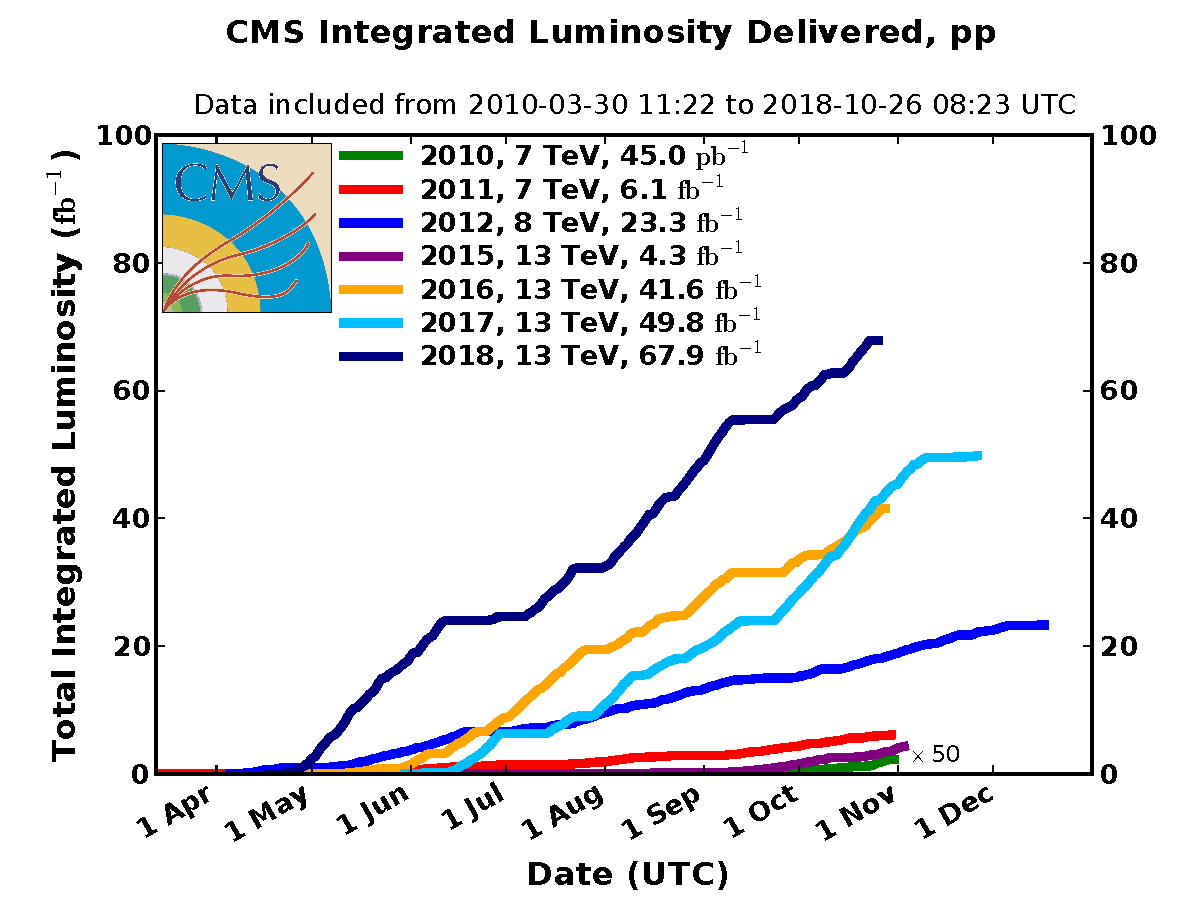
\includegraphics[width=.50\textwidth]{Figures/c2/int_lumi_cumulative_pp_2.pdf}
  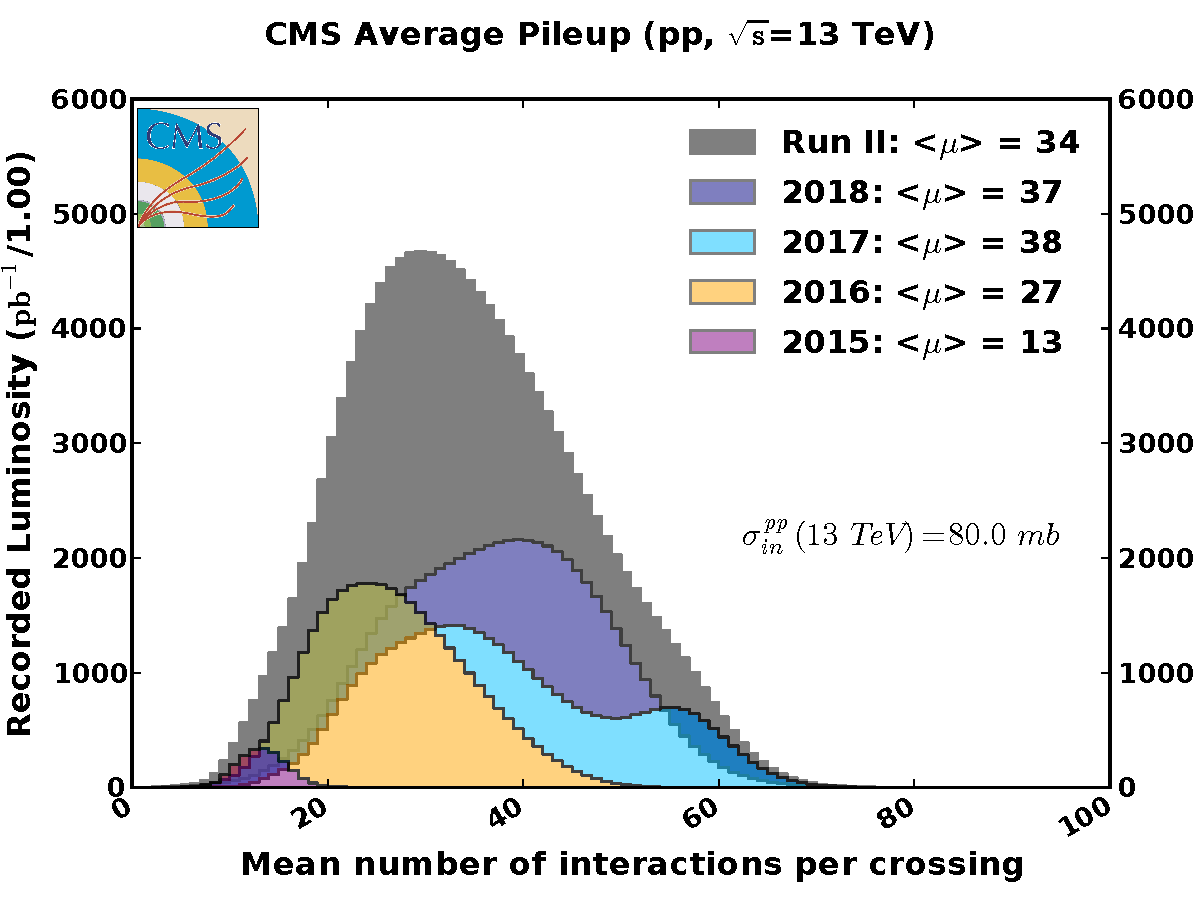
\includegraphics[width=.50\textwidth]{Figures/c2/pileup_allYears_run2.pdf}}\\
  \makebox[\textwidth]{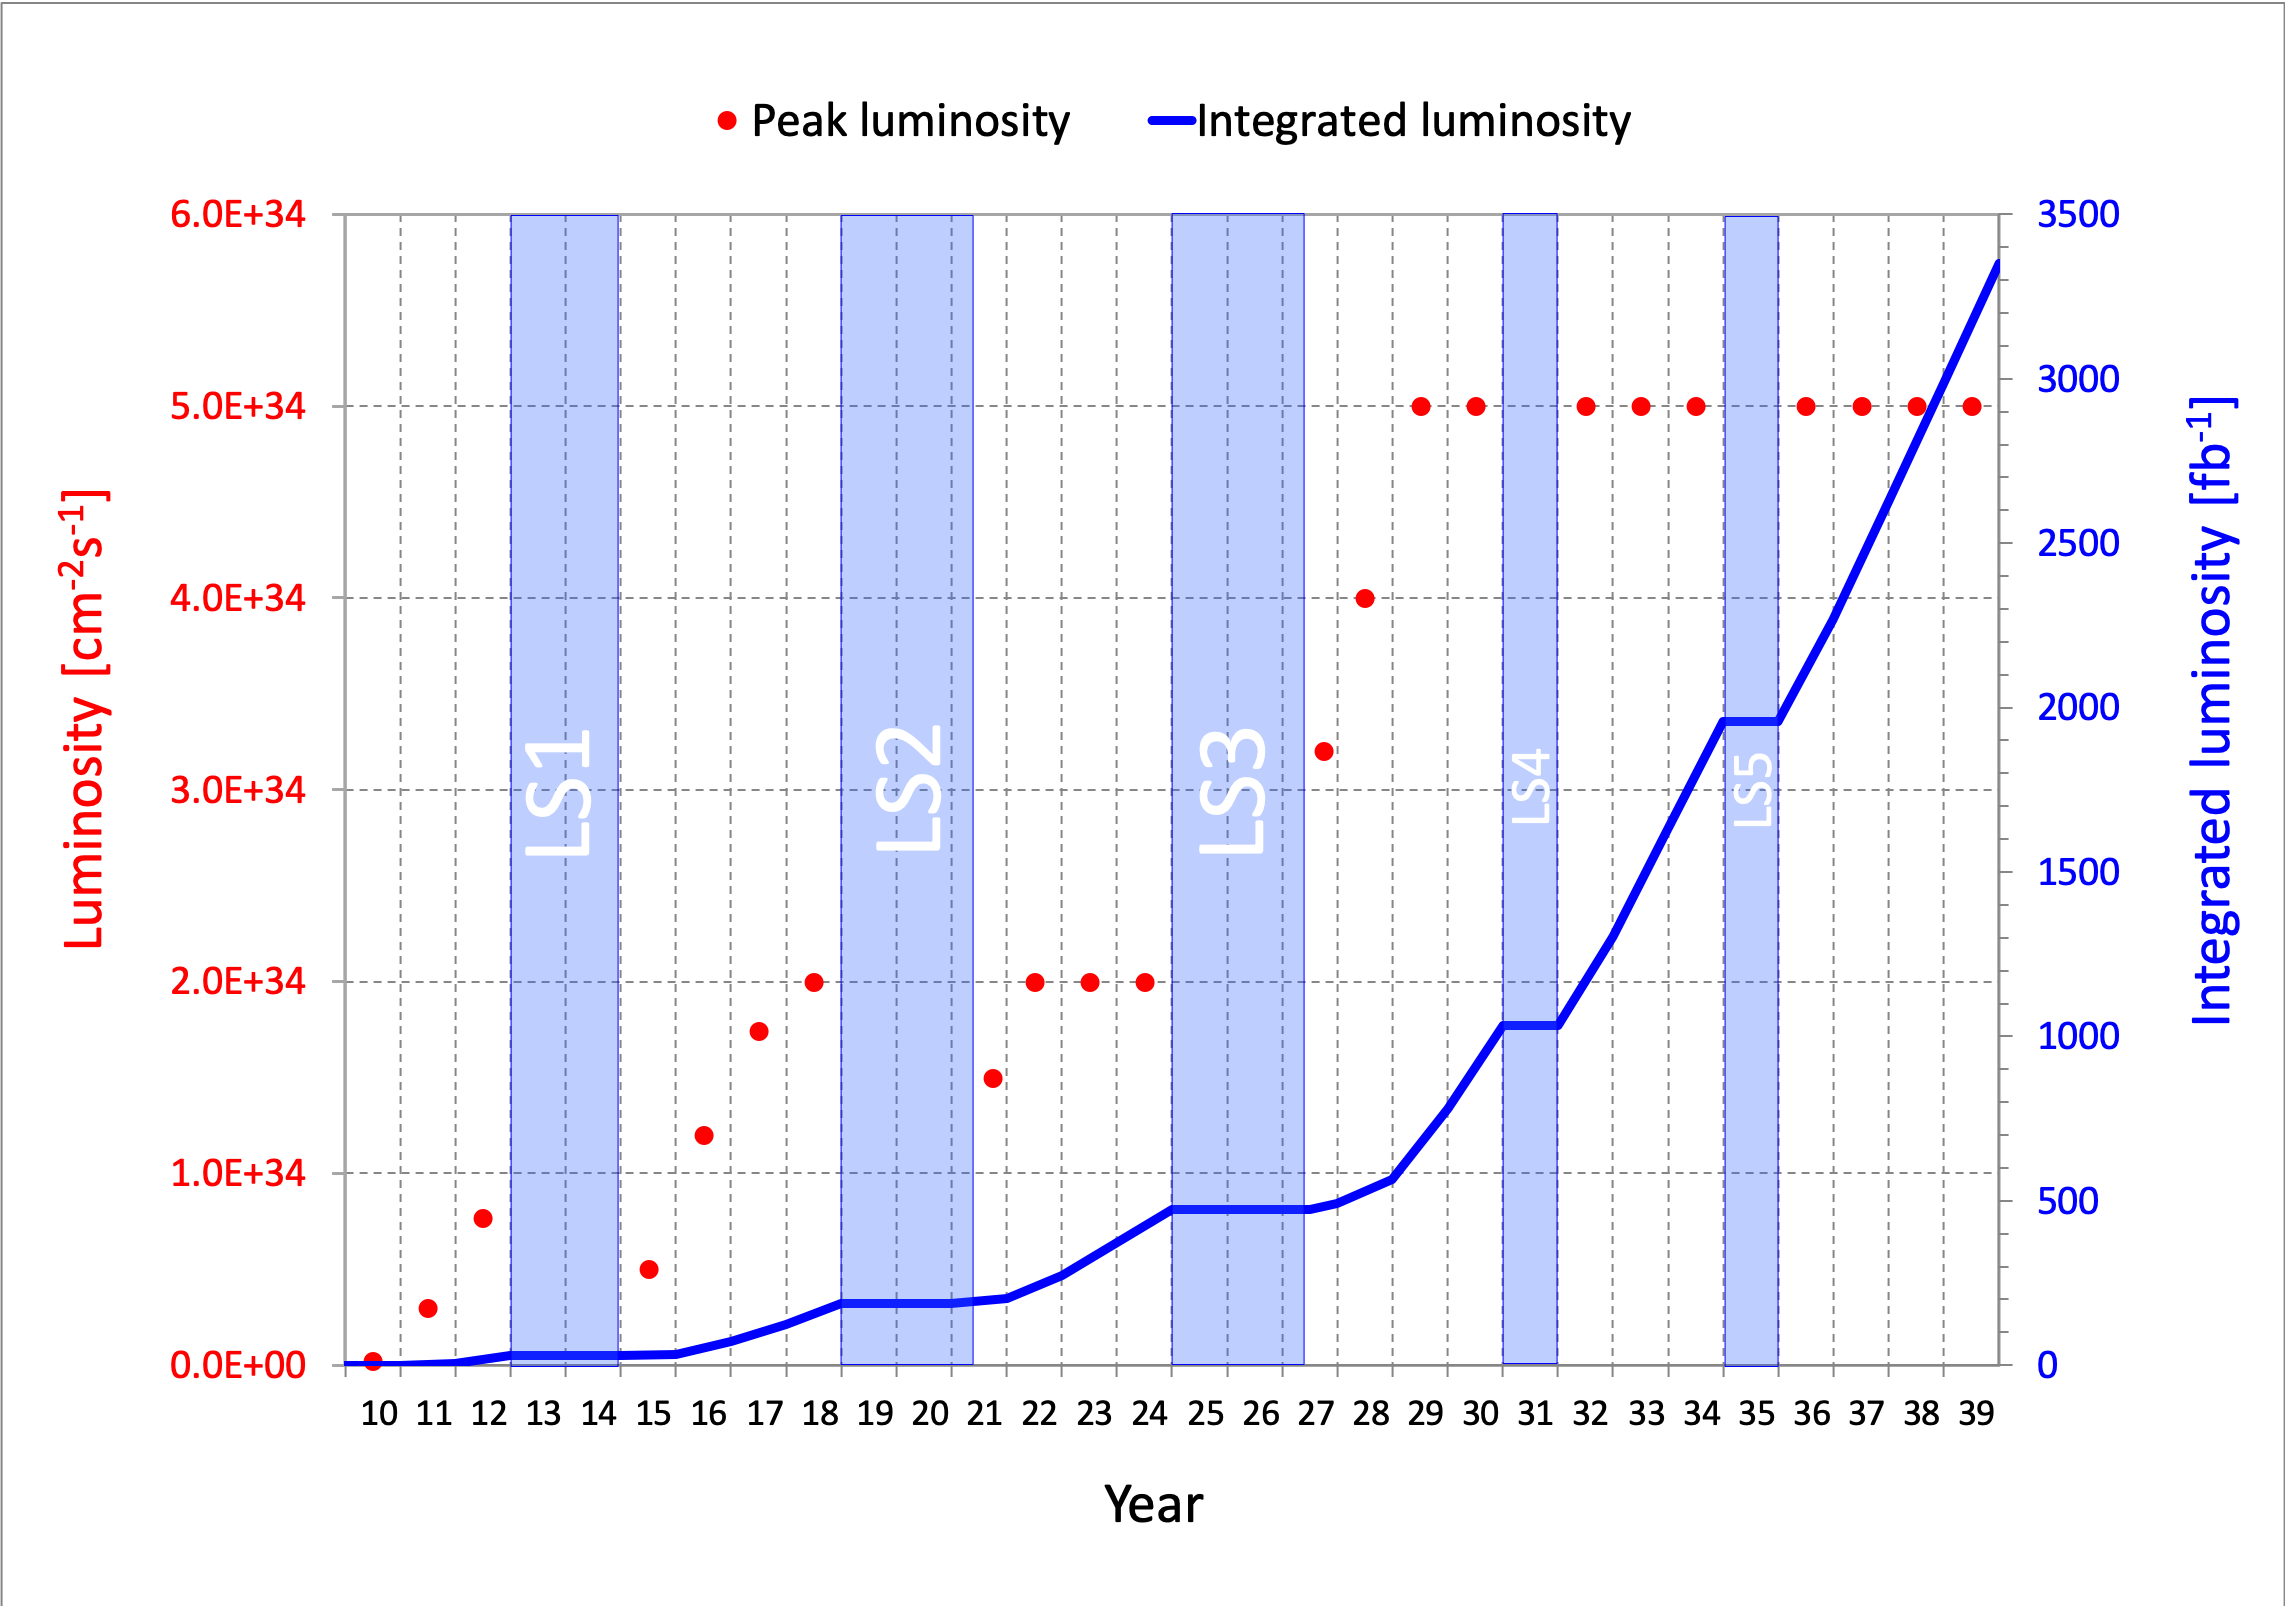
\includegraphics[clip,trim=0.2cm 0.2cm 0.2cm 0.2cm, width=.60\textwidth]{Figures/c2/Lumi.png}}
  \caption{Top-left: integrated luminosity collected by the CMS
    experiment; top-right: distribution of the average number of
    interactions per crossing (pileup) for pp collisions in 2015
    (purple), 2016 (yellow), 2017 (azure), 2018 (periwinkle), and
    full Run2 (gray),~\cite{webpage_lumi}. Bottom: scheduled and
    projected integrated and instantaneous luminosity at the LHC~\cite{webpage_lhc}.}
  \label{fig:lumi}
\end{figure}

The LHC was designed to deliver an instantaneous luminosity
of $10^{34}cm^{-2}s^{-1}$. Figure~\ref{fig:lumi} (top-left and central
plots) shows the schedule of the Large Hadron Collider from the start
to the following years of operations. The LHC has delivered two
outstanding runs of data taking: the first phase, Run1 (2010-2012) at
center-of-mass energy of 7 and 8\TeV and total delivered integrated
luminosity of $29.4\ fb^{-1}$; the first 3 years of data taking proved
the physics potentiality of the LHC with, among others, the Higgs boson
discovery. The second run, Run2 (2015-2018) started after 2 years Long
Shutdown when the machine and the detectors were confirmed and
consolidate to be able to run at the full capacity with 
center-of-mass energy of 13\TeV and total delivered integrated
luminosity of $162.9\ fb^{-1}$.\\
The increase in luminosity over the
years was the result of improvements in the beam quality and optics which
led to an higher number of pp collisions per bunch crossing. This
quantity is referred as pileup, PU which is shown in the top-right plot
in Figure~\ref{fig:lumi}. The average \textlangle{}PU\textrangle{} for
Run2 is 34. On one hand this large
number of collision per bunch crossing 
expands the physics reach of CMS and ATLAS because of
the higher probability of an episode of a rare collision; however
most of the PU interactions pollute the information of the
event being mostly soft and less interesting to look for
new physics models. Thus it is challenging for the detector and the for
the reconstruction algorithms to be able 
to disentangle and reconstruct each single pp collision per single
bunch crossing.

%-----------------------------------
%	SECTION 2
%-----------------------------------
\section{The Compact Muon Solenoid}\label{cms}

The Compact Muon Solenoid (CMS) detector is located at one of the four
collision points along the LHC ring, precisely at LHC P5 in Cessy in
France.  

CMS is a multi-purpose detector designed to observe any new physics
phenomena that could appear at proton-proton collision. CMS behaves
like a high-speed camera capturing instant frames of the particle
collisions up to 40 million times per second. Then by trying to
identify the particles produced and created after the collision,
measuring their energies and momenta the detector aims to recreate a
photograph of the collision for offline analysis. \\
The idea behind the design was to create, around the place where the
two proton beams cross each-other, a structure of concentric cylindrical layers
in order to be able to track and measure the path of the particle
escaping from the center.   

\subsection{The CMS coordinate system} 
The coordinate system used by CMS is a right-handed system defined
locating its center in
\begin{wrapfigure}{r}{0.5\textwidth}
  \begin{center}
    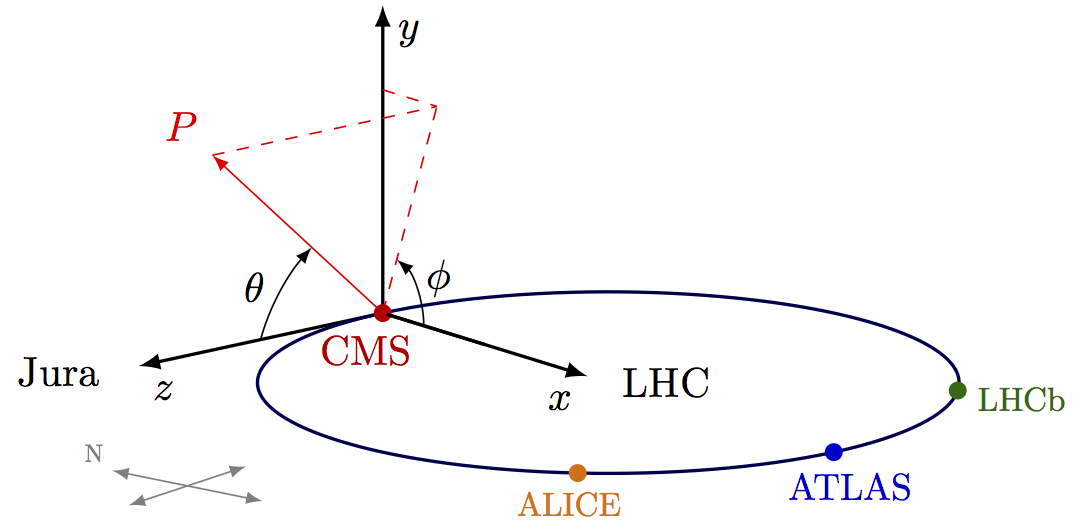
\includegraphics[clip,trim=0cm 0cm 0cm 0.1cm, width=0.48\textwidth]{Figures/c2/cms_coordinate_system.png}
  \end{center}
  \caption{A scheme of the coordinates system used by CMS~\cite{coordinate_cms}.}
\label{fig:coordinates}
\end{wrapfigure}
 the nominal interaction point, the
\emph{y}-axis is vertical pointing upwards, the \emph{x}-axis is
radial pointing inward towards the center of the LHC ring and the
\emph{z}-axis coincides with the direction of the beam
(counter-clockwise beam); refer to
Figure~\ref{fig:coordinates}. The azimuthal angle $\phi$ is defined
from the \emph{x}-axis in the \emph{x-y} plane and the polar angle
$\theta$ is measured from the \emph{z}-axis in the same transverse
plane meaning \emph{x-y} plane.\\
For an object of energy $E$ and momentum $\overrightarrow{p}$,
rapidity, $y$ and pseudorapidity, $\eta$ are defined as:
\begin{equation}
\label{eq:pseudo}
y \: = \: \frac{1}{2} \ln \frac{E + p_z}{E - p_z} \;\; \approx \;\;
\eta \: = \: \frac{1}{2} \ln \frac{|\overrightarrow{p}| +
  p_z}{|\overrightarrow{p}| - p_z} \: = \: -\ln \tan (\frac{\theta}{2})
\end{equation}
The approximation of the rapidity with the pseudorapity is possible for
relativistic particles with $p_{T} \gg m$. The rapidity is used to
measured the angular distance between particles, $\Delta R =
\sqrt{\Delta y ^2 + \Delta \phi ^2}$ which is Lorentz invariant under
boots along $z$-axis the beam direction. Knowing the approximation above,
the $\Delta R$ quantity is often defined as $\Delta R =
\sqrt{\Delta \eta ^2 + \Delta \phi ^2}$.\\
Finally, using the $x$ and $y$ components, the transverse variables
are defined: the transverse momentum, $p_T$ and the transverse energy,
$E_T$.


\subsection{CMS detector}\label{sec:cmsdetector}
The schematic representation of the CMS detector and its parts is
shown in Figure~\ref{fig:detector}.
\begin{figure}[h]
\centering
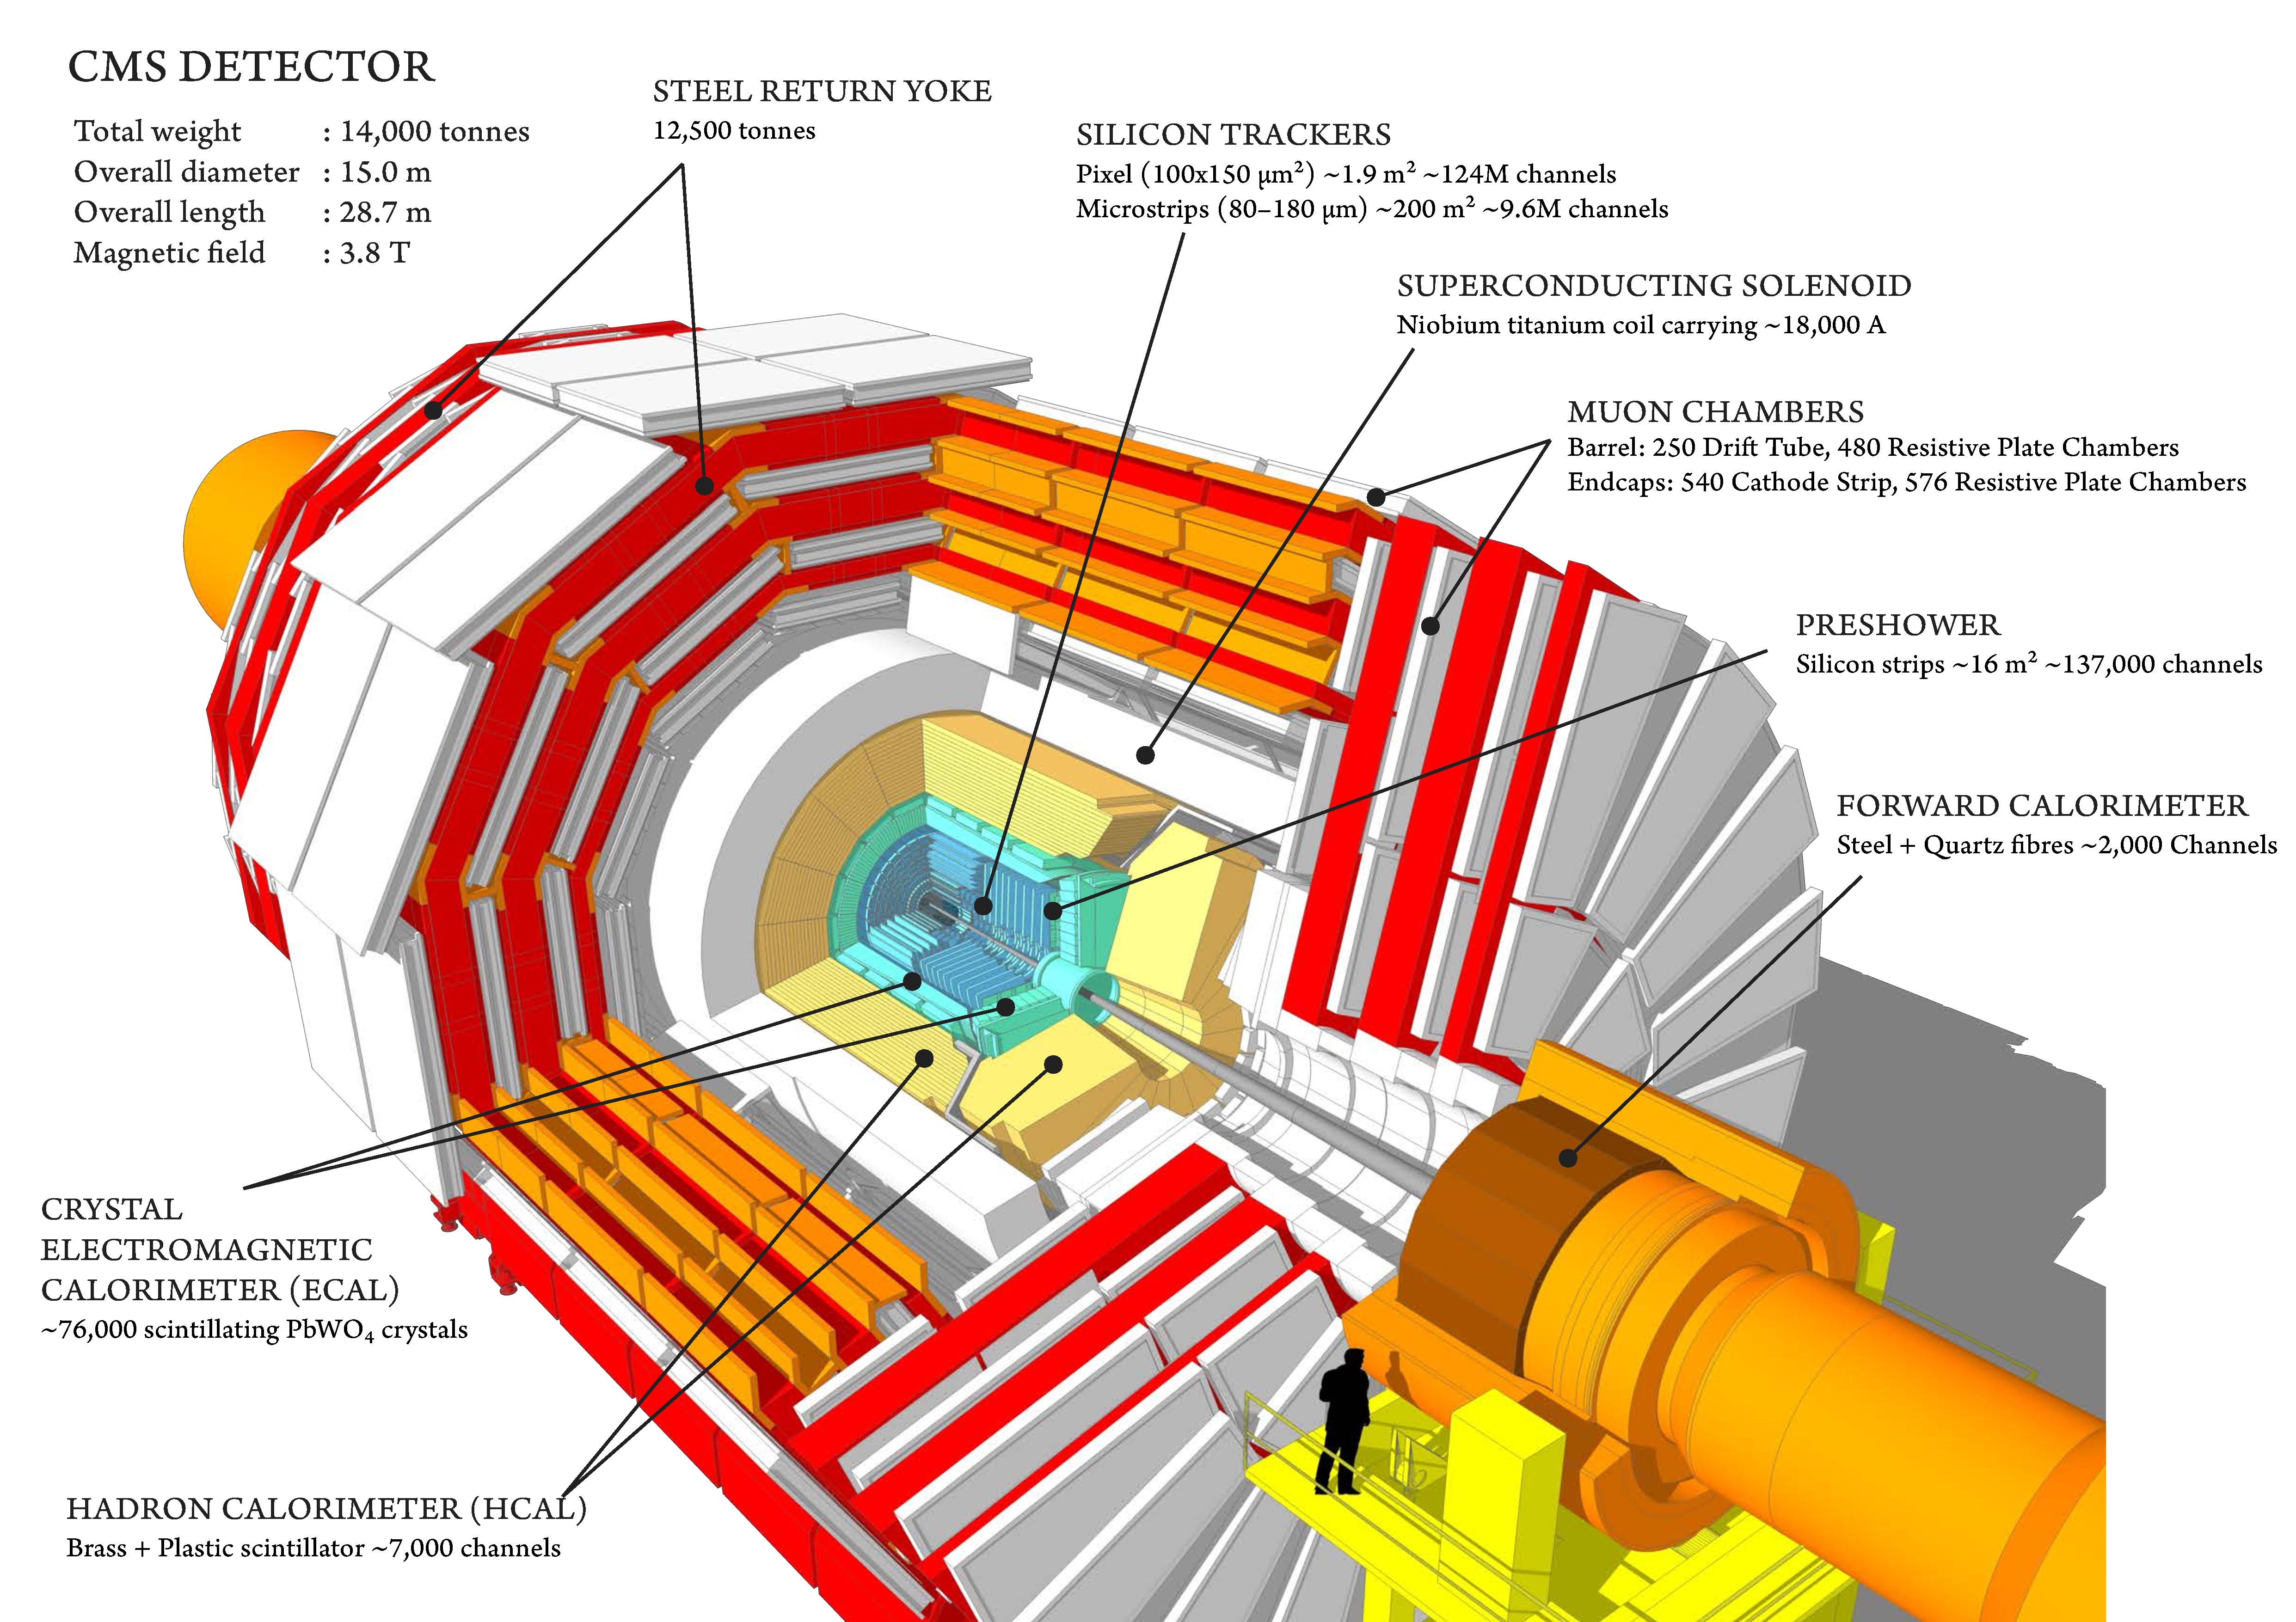
\includegraphics[width=0.98\textwidth]{Figures/c2/cms_160312_06-compressed.pdf}
\vspace*{3mm}
\caption{A scheme of the CMS detector and its parts~\cite{webpage_cms}.}
\label{fig:detector}
\end{figure} 

With CMS detector is possible to measure photons, electrons, muons and hadrons (neutral and charged). 
To be able to achieve such results, CMS is made of a system of sub-detectors each of which contributes with
measurements of specific properties and quantities of different 
particles; the overlap and combination of all the
informations from the sub-detectors allow to identify and measure the
properties of the particles produced during the collision~\cite{Sirunyan_2017}. Beginning
with the region at the immediate proximity to the interaction point, a
particle meets first the tracker where its trajectory, if charged, is
measured. This measure is possible thanks to the presence of the
magnetic field, created by the solenoid, which bends charge particles
and thus tracks reconstruction provides insight on electric charge and
momenta of the particle itself. Subsequently there are the
electromagnetic (ECAL) and hadronic (HCAL) calorimeters where
electrons/photons and hadrons are receptively absorbed and their
energies measured. Finally the muons, getting through the
calorimeters, enter into the muon chambers where complete trajectory
is then measured. 

The subsystems of the CMS experiment are listed and briefly described
in the following paragraphs.

\subsubsection{The superconducting solenoid}
The central part of CMS is a solenoid magnet of 6 m internal diameter
which is made of a cylindrical coil of superconducting fibers
providing a magnetic field of 3.8 T. 
\subsubsection{The tracking system}\label{sec:tracking}
The design of the CMS tracking system is optimized to
efficiently and precisely measure the trajectories of charged
particles and to effectively reconstruct secondary vertices. This latter feature is of particular
importance in the context of displaced vertices and lepton searches as
described in Chapter~\ref{Chapter6}.

\begin{figure}[h]
\centering
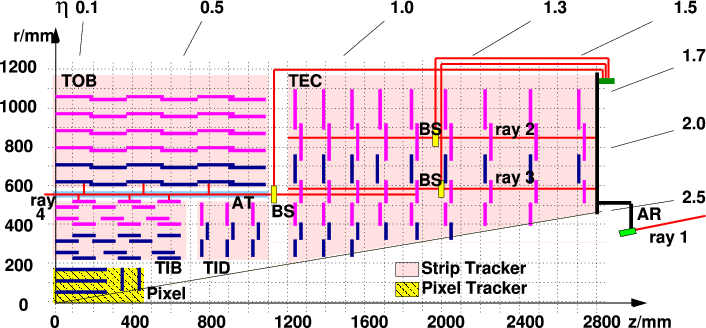
\includegraphics[width=0.98\textwidth]{Figures/c2/las}\\
\vspace{0.5cm}
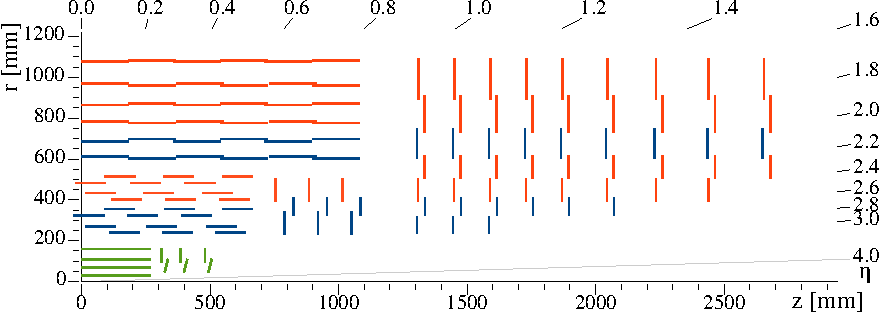
\includegraphics[width=0.68\textwidth]{Figures/c2/Phase1_Tracker_1Quarter.pdf}

\caption{Top: a quarter of the CMS silicon tracker in an $r-z$
  view. The strip tracker comprises several parts: the tracker inner
  barrel (TIB), outer barrel (TOB), inner disks (TID) and endcaps
  (TED)~\cite{Adam:1171503}. Bottom:
sketch of one quarter of the current CMS tracking system in
  r-z view, 2017-2018 data taking. The pixel detector is shown in
  green with the additional modules~\cite{trackingPU}.}
\label{fig:tracker}
\end{figure} 
Additionally the tracking system has to feature high granularity and
fast response in order to correctly associate each reconstructed track
to the respective bunch crossing and the primary interaction vertex.

The CMS tracker consists of a pixel detector (pixel Tracker) and a
silicon strip detector (strip Tracker), see Figure~\ref{fig:tracker}.
The original pixel detector was made of three barrel
layers at radii of 4.4, 7.3, and 10.2 cm and two endcaps modules in
the forward region. 
During the short shutdown between the data takings 2016 and 2017, it
was installed an
upgraded version of the pixel detector; the detector has currently four
barrel layers at radii of 3.0, 6.8, 10.2, and
16.0 cm and three layers in the forward region~\cite{Dominguez:1481838}. The
recent innermost layer and modules
are positioned closer to the beam pipe in order to improve the
precision on the position of the interaction vertices.\\
The silicon strip detector consists of many parts: the tracker inner and
outer barrels (TIB and TOB), in total ten layers of strip modules in
the barrel; the 6 tracker inner disks (TID), three each
side; and the nine disks on each side of the tracker endcap (TEC).\\
In total the tracking system is 5.8 m long and 2.6 m high,
extending the coverage of the tracker up to $|\eta|$ = 2.5. The total
amount of sensors is 66 million for the pixel and 124 million for the
strip detector. 

\subsubsection{The electromagnetic calorimeter}
The ECAL detector is a fine-grainded and homogeneous calorimeter
made up of lead
\begin{wrapfigure}{r}{0.5\textwidth}
  \begin{center}
    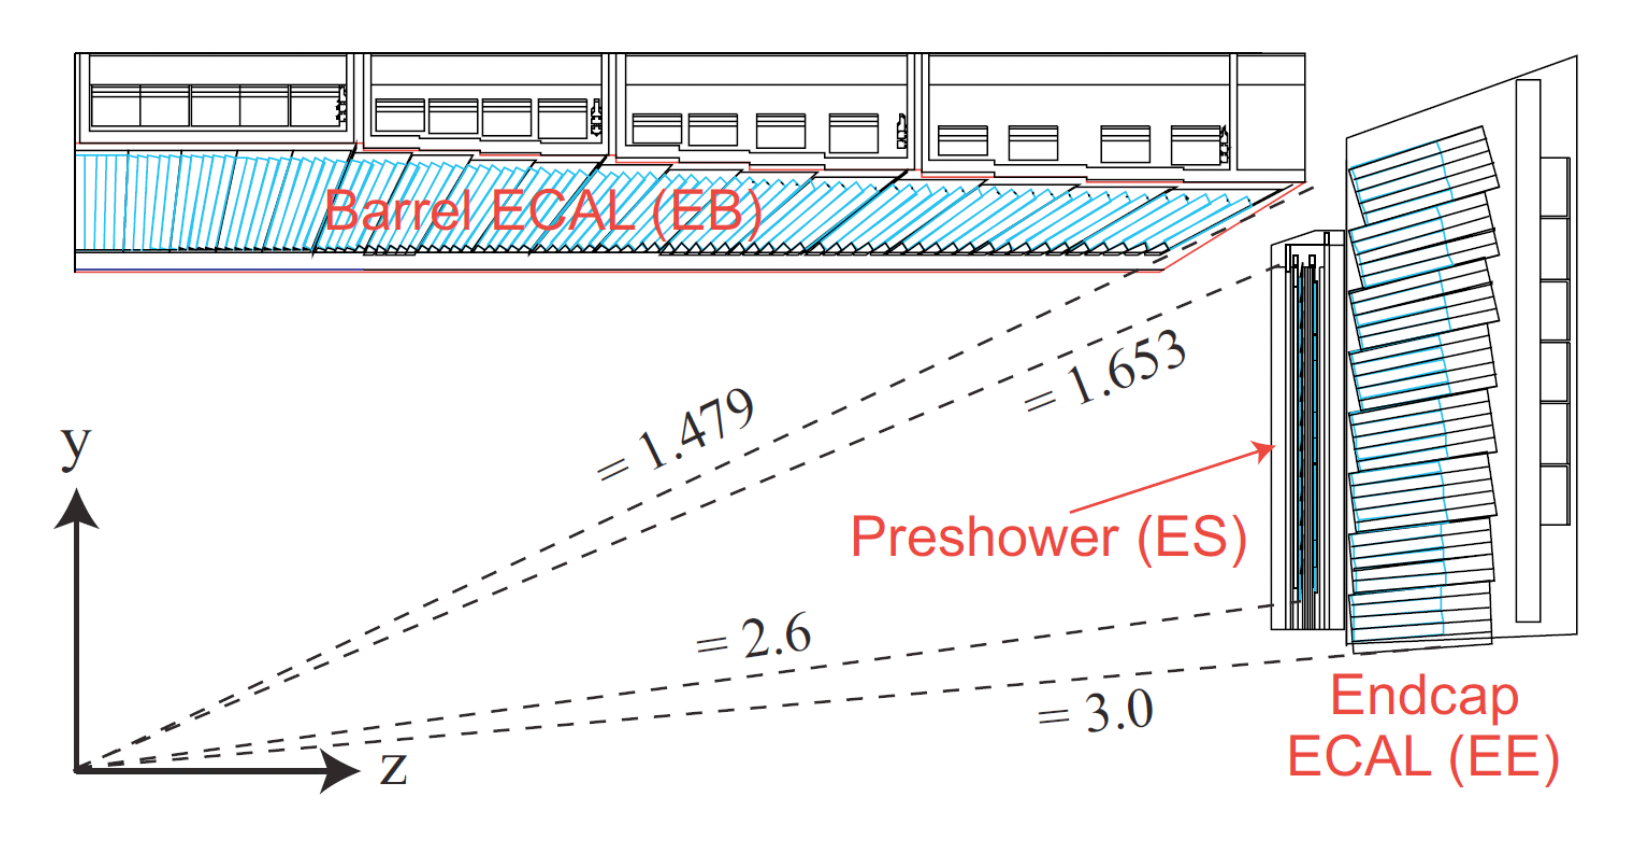
\includegraphics[clip,trim=1cm 1cm 1cm 1.5cm, width=0.48\textwidth]{Figures/c2/ecal}
  \end{center}
  \caption{Geometric view of one quarter of the ECAL~\cite{Benaglia_2014}.}
\label{fig:ecal}
\end{wrapfigure}
 tungstate crystals. Those single crystals are extremely transparent
 and ``scintillates''  when photons and electrons pass through
 them; the light produced is proportional to the particle's energy
 allowing a fast and very precise measurement of the momentum
 property. The single crystal length in barrel region is 230 mm (220
 mm in endcap) comparable to $\sim$26 (25) radiation lengths meaning it
 absorbs more than 98\% of the energy deposited by the particle~\cite{Biino_2015}.\\
A scheme of the ECAL is shown in Figure~\ref{fig:ecal}.
ECAL modules are placed in the barrel ($\eta<$ 1.479) and endcap
(1.635 $<\eta<$ 3.0) regions, and a preshower detector is located just
before the endcap crystals. The preshower detectors help CMS to
distinguish between single high-energy photons and the less
interesting pairs of low-energy photons very close to each other, \ie
coming from the decay of a $\pi^0$. 

\subsubsection{The hadron calorimeter}
The HCAL detector is a hermetic sampling calorimeter which means it
consists of alternative layers of ``absorber'' and ``scintillator''
materials that measure a particle’s position, energy and arrival time.
The quantity of light in a given position is summed up over several
layers of tiles in depth, called a “tower”, thus this total amount of
light is a measure of a particle’s energy.\\
The HCAL is located both inside the solenoid, the main part, and
outside it, the outer barrel (HO). 
Inside the magnet coil, the barrel (HB) and endcap parts (HE) cover
respectively the pseudorapidity
ranges $\eta<$ 1.3 and 1.3 $<\eta<$ 3.
The forward region of pseudorapidity is covered by the forward hadron
calorimeter (HF) up to $\eta<$ 5. It is made up of iron radiators and
quartz-fibre sensors and it measures both the electromagnetic and the hadronic shower. 
The outer barrel, HO, ensures no energy leaks out the
back of the HB undetected.

\subsubsection{The muon system}\label{sec:muonsystem}
The muon system is constructed to detect muons and to measure their trajectories.\\ 
It is composed by three different kind of gaseous particle
detectors inserted in the steel yoke. There are the drift tubes
modules, DTs, the cathode strip chambers, CSCs and the resistive plate
chambers, RPCs.\\
The four layers of DTs are located in the barrel and they cover up to
$\eta<$ 1.2 pseudorapidity range in the detector. The four layers of
CSCs are installed in the endcap covering the pseudorapidity range 0.9
$<\eta<$ 2.4. Finally there are the RPCs positioned both in barrel
and endcap parts up to $\eta<$ 1.6. The whole pseudorapidity range of
the muon system allow to measure muons up to $\eta<$ 2.4.

\begin{figure}[h]
\centering
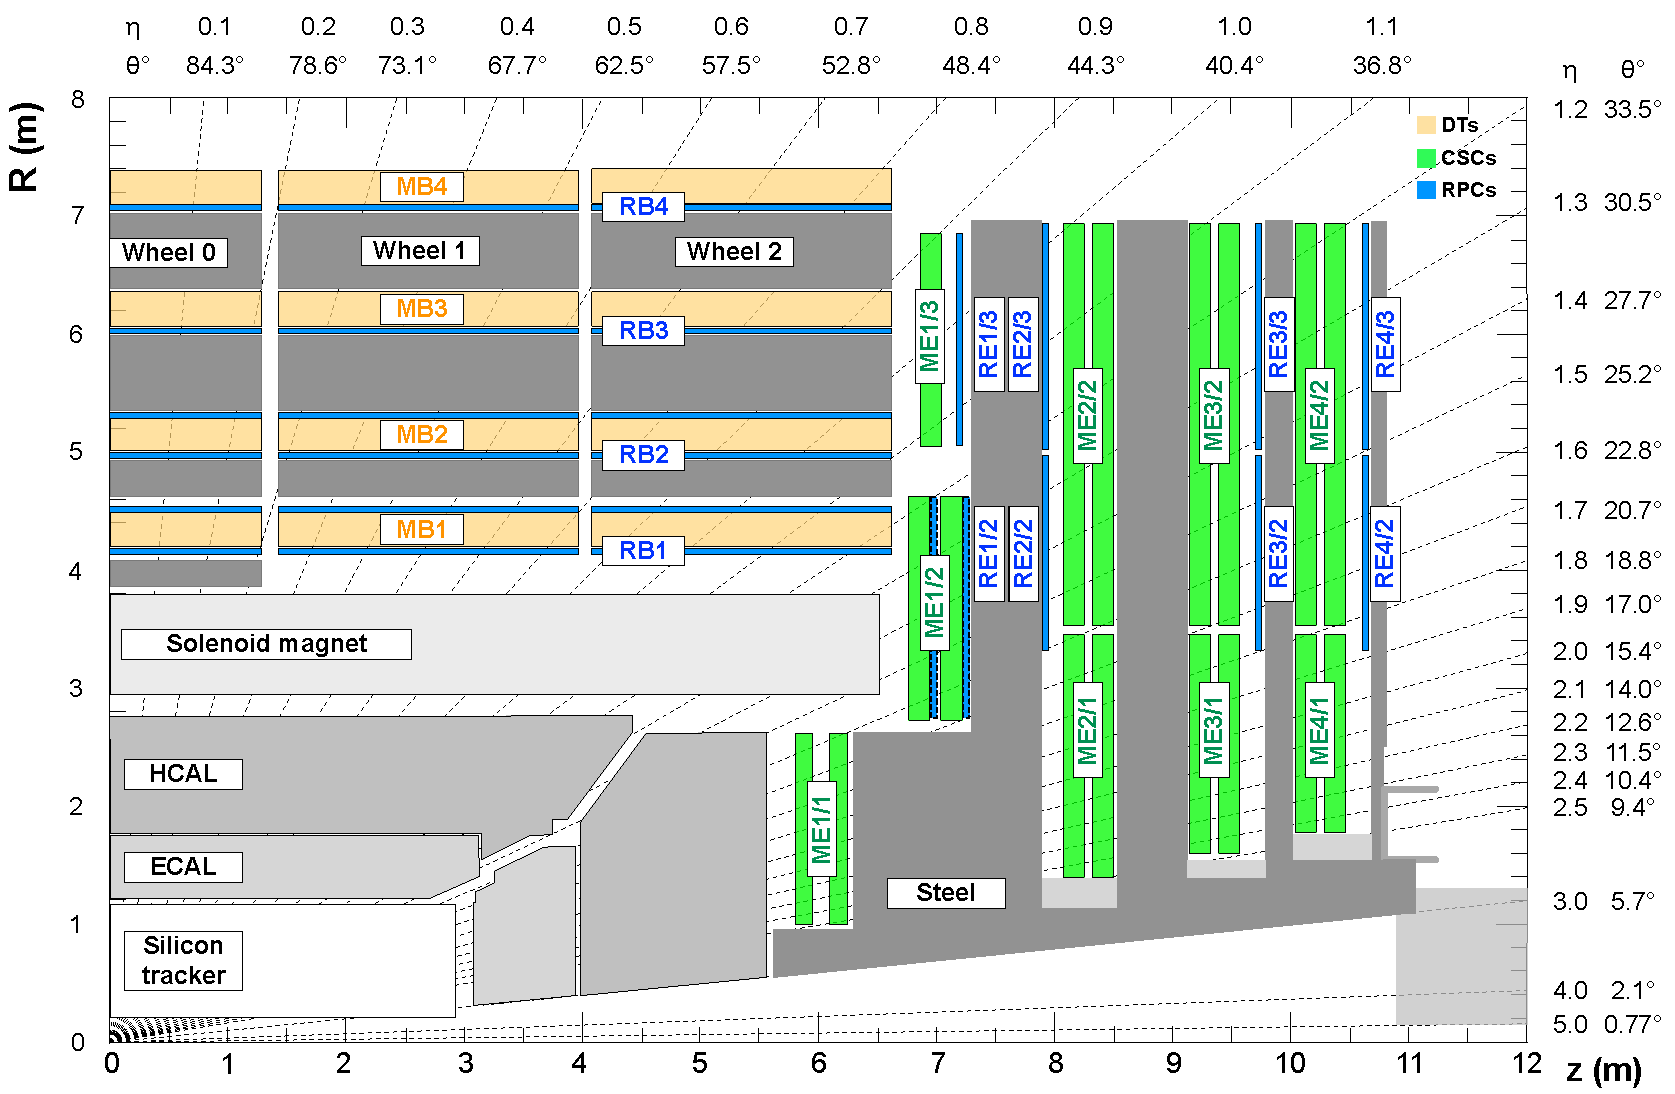
\includegraphics[width=0.98\textwidth]{Figures/c2/cms_quadrant_run_ii.pdf}
\caption{Geometric view of one quadrant of CMS. The grey areas are
  tracker, ECAL and HCAL systems, previously explained; the colored
  areas show the muon system and its subsystem. The drift tube, DTs,
  modules are labelled MB (muon barrel) and the cathode strip
  chambers, CSCs, are labelled ME (muon endcap). Resistive plate
  chambers, RPCs, are labelled RB and RE and they are mounted in both the barrel and endcaps of CMS
~\cite{muonsystemPU}. }
\label{fig:muonsystem}
\end{figure} 

\subsubsection{The CMS trigger system}\label{sec:triggersystem}

At center of the CMS detector, proton-proton collisions occur every
25 ns which means a frequency of 40 MHz. However not every collision is
necessarily of potential interest for the CMS physics program and
moreover there are technical limitations on the rate the collision data can be
saved on disk to be analyzed offline. Thus a trigger is needed to be
able to sort between potentially interesting events and the extent of
inelastic scattering events.
Since the reading and storing time of the collision data is larger
than the collision frequency the viable solution is
to store the informations in pipelines that hold and process data
from several collision at the same time.
To work without mixing particles from two different events, it is
required detectors have very good time
resolution and the signal from the millions of channels of different
systems to be synchronized and integrate.

The CMS trigger has a two-stage architecture. The first level, L1 is
implemented in custom hardware and uses informations from the 
all muon systems and the calorimeters to identify events applying a fast
basic identification of measured particles. The first step reduces the
event rate to $\sim$100 kHz.\\
The events sorted by the L1 are further refined by the
high-level trigger, HLT. It is a software farm that employs informations from all sub-detectors to perform a
refined event reconstruction reducing the rate down to a few kHz. The 
events are then saved for offline analysis.
The trigger selection is a irreversible process, what was not selected
by it is lost and it can not be recovered~\cite{Khachatryan_2017}.

A complete sequence of L1
and HLT selection criteria, including any prescale, is referred to
as a trigger path.

\clearpage
%-----------------------------------
%	SECTION 2
%-----------------------------------

\section{Event reconstruction}\label{sec:reconstruction}
With the term ``event reconstruction'' is meant the identification of
all final state particles which are produced in a proton-proton
collision. Particles are classified according to their distinct
signatures they present in 
the CMS detector, as displayed in Figure~\ref{fig:cmsslice}.

CMS detector is built with the idea of cylindrical detection layers
which are wrapped around the beam axis. After the collision, starting
from the point where the interaction occurred, particles enter in the
tracker. In the tracker charged-particle trajectories, \emph{tracks}
and origins, \emph{vertices} are reconstructed using the information from
electronic signals, \emph{hits}, in the detection layers. Subsequently
electrons and photons are absorbed in the ECAL where they stop, and
charged and neutral hadrons could start a hadronic shower in the ECAL
already and being fully absorbed in the HCAL. Muons and neutrinos cross
the full detector with little or zero interactions; the muons reaching the muon-system produce
signal hits and they trajectory is finally defined. This simple
event-view is graphically displayed in Figure~\ref{fig:cmsslice}.
\begin{figure}[h]
\centering
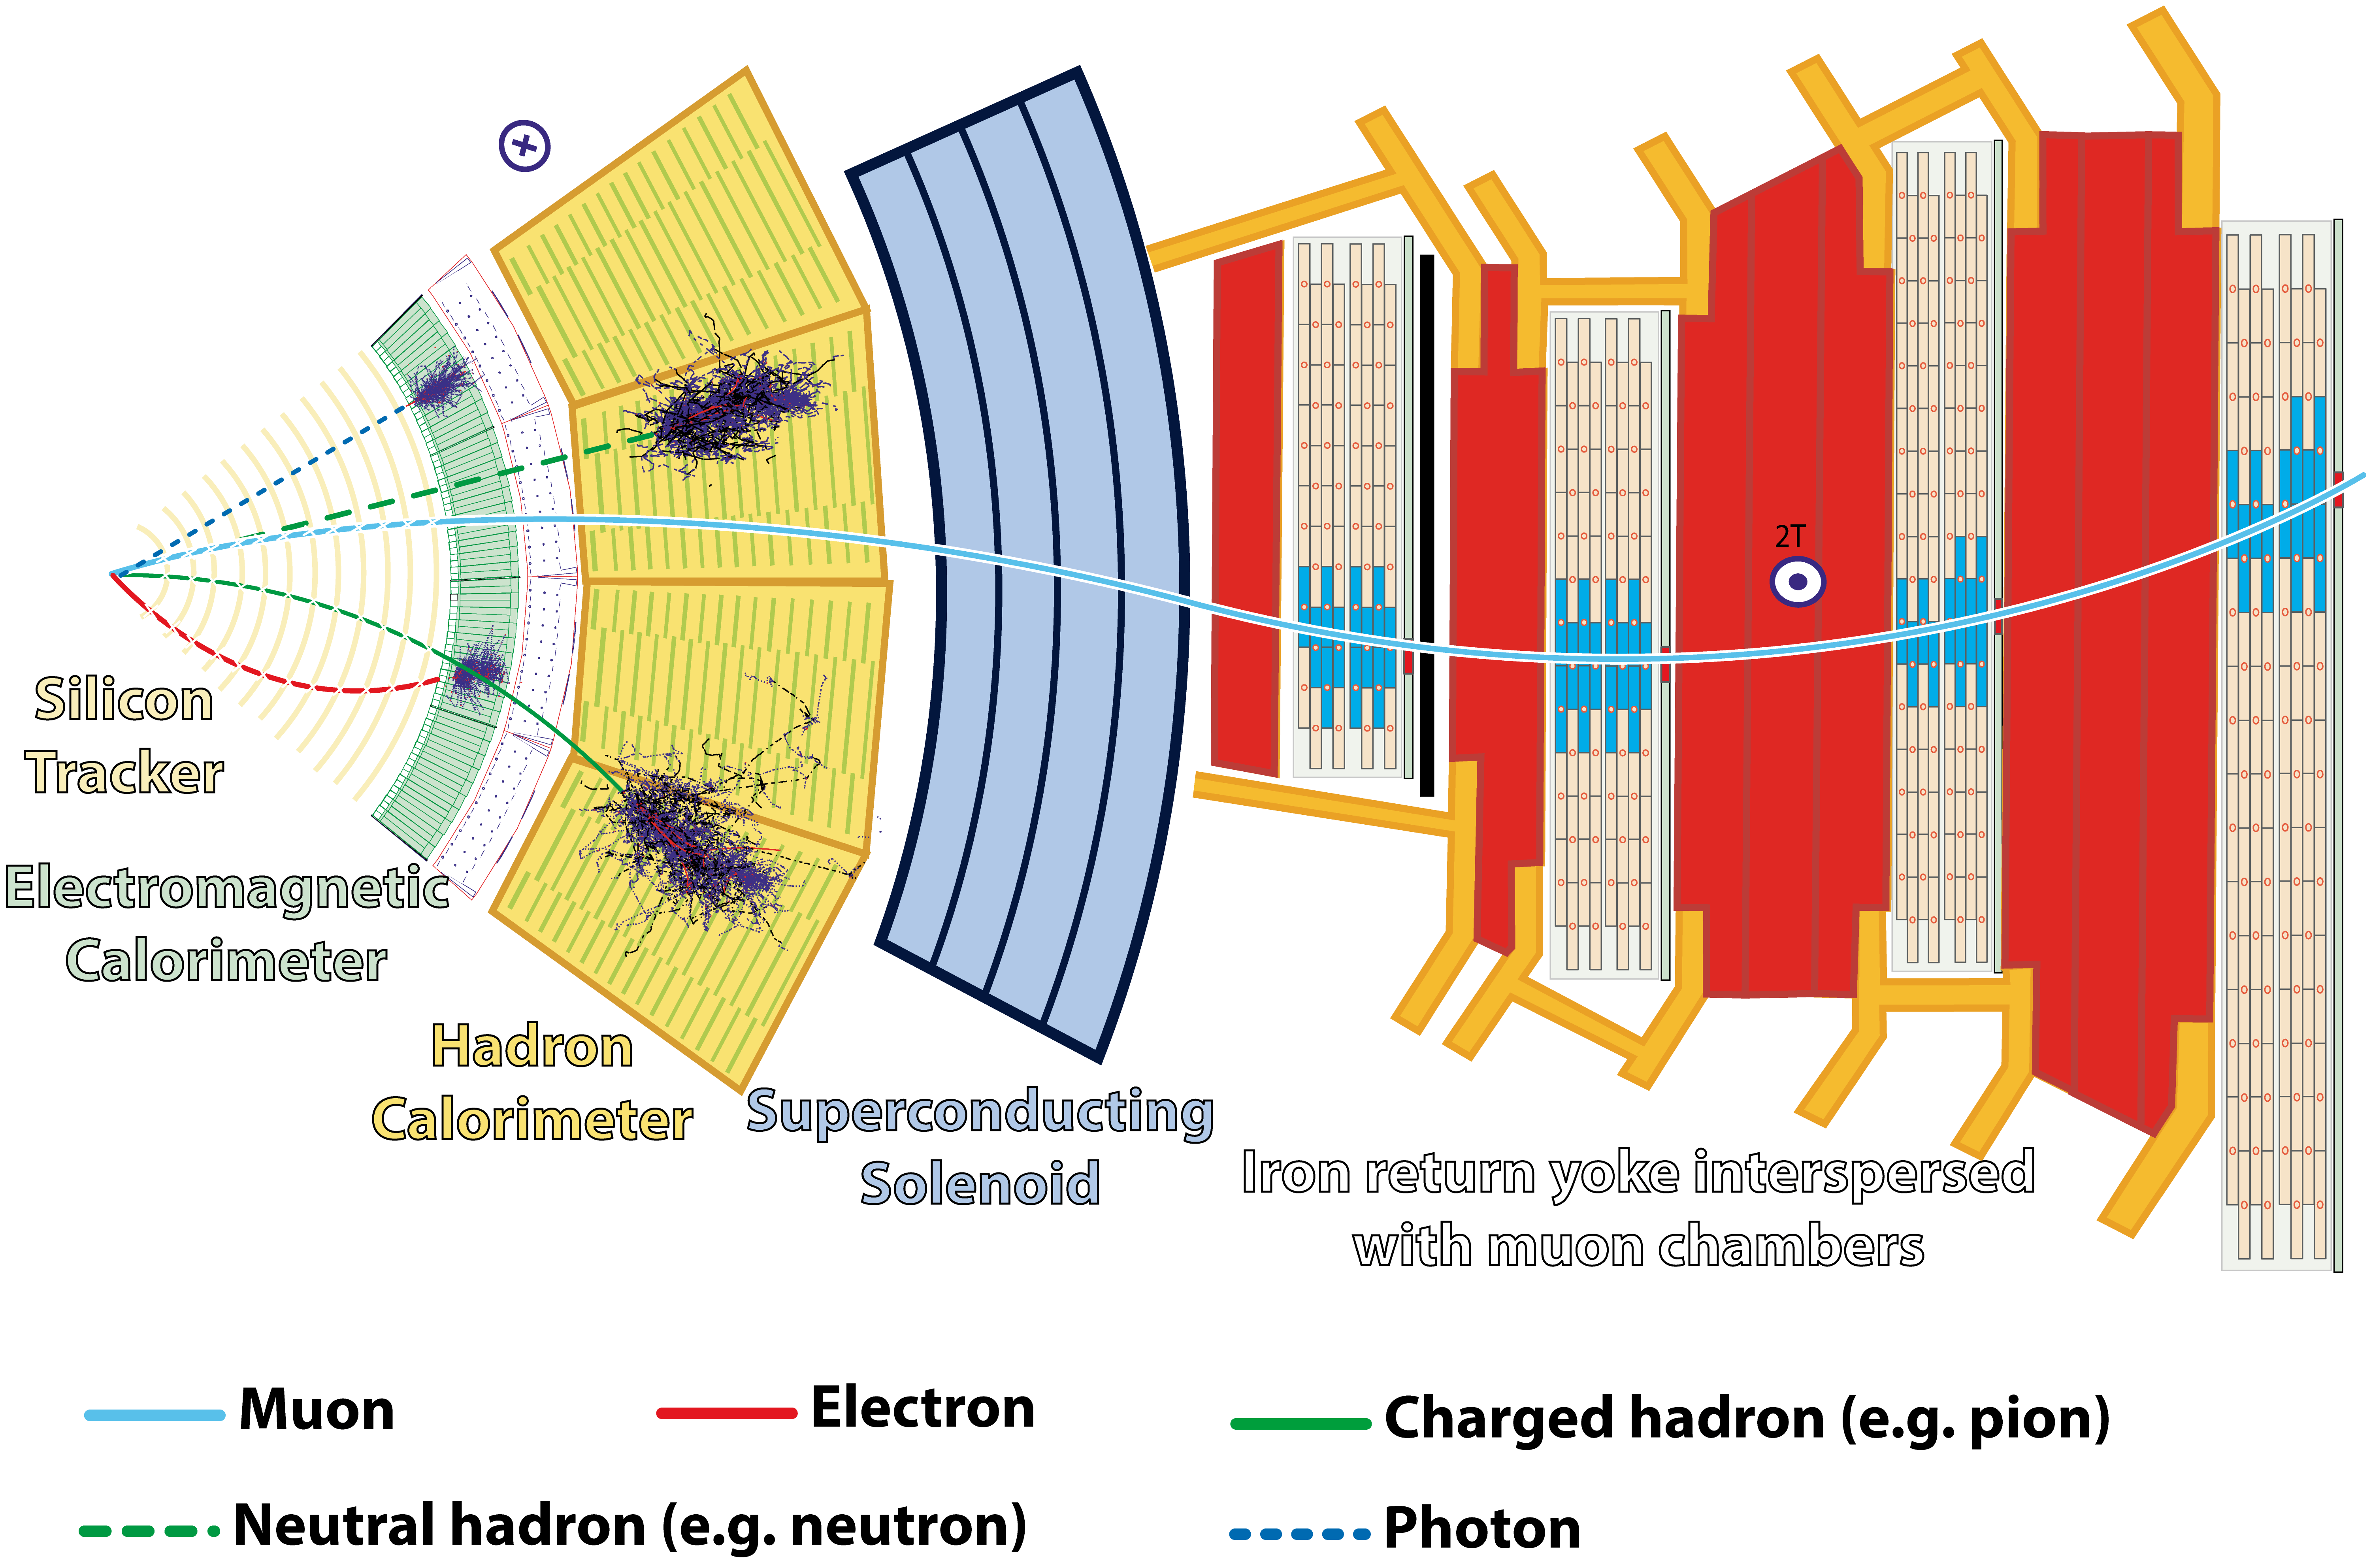
\includegraphics[width=0.78\textwidth]{Figures/c2/CMSslice.png}\\
\caption{Geometric view of a transverse slice of the CMS detector showing its sub-detectors and how particles interact with them~\cite{Barney:2120661}.}
\label{fig:cmsslice}
\end{figure} 

This approach has led to the practice of reconstructing \emph{physics
objects} in the first place using the signals collected by a specific
detector in the following way:
\begin{itemize}
\setlength\itemsep{-0.2em}
\item \emph{jets} (hadron and photons): the energy can be measured by ECAL
  and HCAL without any try to divide individual jet particles. Jet
  reconstruction can happen without the input from the tracker. The
  same idea applies to the \ptmiss;
\item \emph{isolated photons and electrons}: the reconstruction interests the
  ECAL;
\item \emph{jet tagging}: it is possible tag jets with origin from hadronic $\tau$ decay and
  from b quark hadronization. The tagging makes use of the properties of
  the related charged particle tracks, hence mostly concerns the
  tracker;
\item \emph{muons}: the identification is primarily based on the information
  from the muon-system.
\end{itemize}

An additional improvement on the event description is obtained by
correlating (\emph{linking}) the basic \emph{elements} (\ie tracks and
clusters) from all the sub-systems to classify each final-state
particle and then by combining the measurements to be able to
reconstruct the physics-object properties like mass and momentum. This
integrated approach is called \emph{particle flow} (PF)
\emph{reconstrution}~\cite{CMS:particleflow} and it is going to be
explained later in Section~\ref{sec:PF}.




This chapter details the approach and the relevant steps of the CMS
event reconstruction algorithms, paying particular attention to the
aspects pertinent to this thesis (i.e. light leptons). The track and vertex reconstruction 
is presented in Section~\ref{sec:trackvertex} and particle-flow
algorithm is described in Section~\ref{sec:PF}. Identification and
performances of muons and electrons are presented in
Sections~\ref{sec:trackmuon} and~\ref{sec:trackele}.


\subsection{Track and vertices reconstruction}\label{sec:trackvertex}

Be able to precisely reconstruct interaction vertices and charged
particle tracks is a crucial element for an accurate measurement of
charged particle momenta and properties. Tracks, vertices and their
successive combination constitute an important input for pileup
mitigation (Section~\ref{lhc}) and for the
identification displaced vertices from which particles from long-lived
particle decay originate.
Lastly tracks and vertices are fundamental inputs to the particle-flow (PF) algorithm (Section~\ref{sec:PF}).\\
The tracking algorithms are devised to
increase the track-finding efficiency while keeping small the
contamination of fake tracks, \ie tracks constructed from uncorrelated hits or
including false hits.\\
 
The tracks are reconstructed starting from the hits in the pixel and
strip tracker. The hit reconstruction follows two steps: the first,
indicated as local reconstruction, is a clustering of signals in the
tracker sensors. Thus 
the first estimate of the
position of the hit is determined based on the geometry of the single
pixel or strip while taking into consideration the Lorentz drift due
to the magnetic field (more detailed info about local reconstruction
can be found here:~\cite{CMS:particleflow}). The second step is a more
sophisticated reconstruction which uses the informations about the
irradiation status of the pixel and strip sensors. \\
The hit efficiency is measured to be above the 99.5\%\footnote{The hit
  efficiency depends on the
$d\mathcal{L}/dt$ and on the trigger rate, in particulars in
the first layer of the pixel sub-detector where the occupancy is greater.} for both pixel
and tracker hits~\cite{CMS:particleflow}. According to the size of the
cluster and the angle of
incidence of the particle, the final resolution in the
hit position is measured to be in the range of 20 (10) and 50 $\mu$m
for the pixel (strip) tracker~\cite{CMS:particleflow}.\\
An additional inputs for the track reconstruction are the identification
of the LHC beam spot position, \ie the LHC luminous region's
3D profile, and the position of the collision
vertices. 

The tracking algorithm used by CMS is called Combinatorial Track Finder (CTF)~\cite{Collaboration_2014_tracking}.
To lower the combinatorial complexity, it is applied an iterative
procedure in distinct successive iterations, each with moderate
efficiency and loosened selection requirements on the track quality with
respect to the step before. The method of Kalman
filter~\cite{BILLOIR1990219} is used for the track-finding
algorithm. While taking into account the multiple Coulomb scattering on the
direction of the track, the Kalman filter makes use of track
seeds\footnote{``\emph{The seeds define the starting trajectory parameters and associated uncertainties of potential
tracks. In the quasi-uniform magnetic field of the tracker, charged particles follow helical paths
and therefore five parameters are needed to define a trajectory. Extraction of these five parameters
requires either three 3-D hits, or two 3-D hits and a constraint on the origin of the trajectory
based on the assumption that the particle originated near the beam
spot}''~\cite{Collaboration_2014_tracking}.} 
to extrapolate the track
trajectory to the successive detector module. Thus at each layer, new
additional consistent hits
are integrated into the trajectory and the track parameters are
calculated again. The procedure starts again and the new resulting
trajectory is extrapolated to the subsequent layer. At the end, tracks
which do not fulfill goodness-of-fit requirements are rejected. Tracks
which are ``easy'' to reconstruct, e.g. from particle with large \pt
(which means less evident curvature) and produced in proximity to the
interaction point, are reconstructed first. Therefore hits associated
to these tracks are taken out making the subsequent iterations less
complex. To guarantee high efficiency, track-finding starts with
trajectory seeds which are built in the innermost region of the
tracker. 
The reconstruction efficiency for tracks with \pt $>$ 1\GeV  is measured to be larger
than 99\% for isolated muons for $|\eta| < $ 2.5 and between 80 and
99\% for electrons and pions~\cite{CMS:particleflow}. The track \pt
resolution depends on the \pt and $\eta$ of the tracks, and it is
lower than 1\% for muons with \pt $\in [1,10]$\GeV~\cite{CMS:particleflow}.

Vertices are reconstructed using the high-quality tracks which are
compatible with originating in the beam spot. They are then clustered
based on their coordinates along the \emph{z}-axis. An adaptive vertex
fitting~\cite{Waltenberger_2007} developed as an iterative re-weighted Kalman filter
is used to estimate the coordinates of the vertices. To each track it is assigned a
weight between 0 and 1 according to the probability for that track to
belong to a specific vertex. Thus vertex weights are appointed to each
vertex as the sum of the weights of all the
associated tracks, and the vertices with weights inferior predefined
thresholds are rejected. The reconstruction efficiency depends on the
number of tracks associated to the vertex and it is estimated to
be close to 100\% for the cases with more than two tracks and around
98\% for vertices with two tracks~\cite{CMS:particleflow}. The
resolutions varies between 10 and 100 $\mu$m~\cite{CMS:particleflow}.\\
The primary vertex (PV) is identified as the vertex with the largest $p^2_T$ sum for
physics-objects associated to it. The other vertices are assigned as pileup
vertices.

\subsection{The particle-flow algorithm}\label{sec:PF}

The PF algorithm~\cite{CMS:particleflow} is devised to cater a global event
description by linking and combining information from CMS
sub-detectors. 
\begin{figure}[h]
\centering
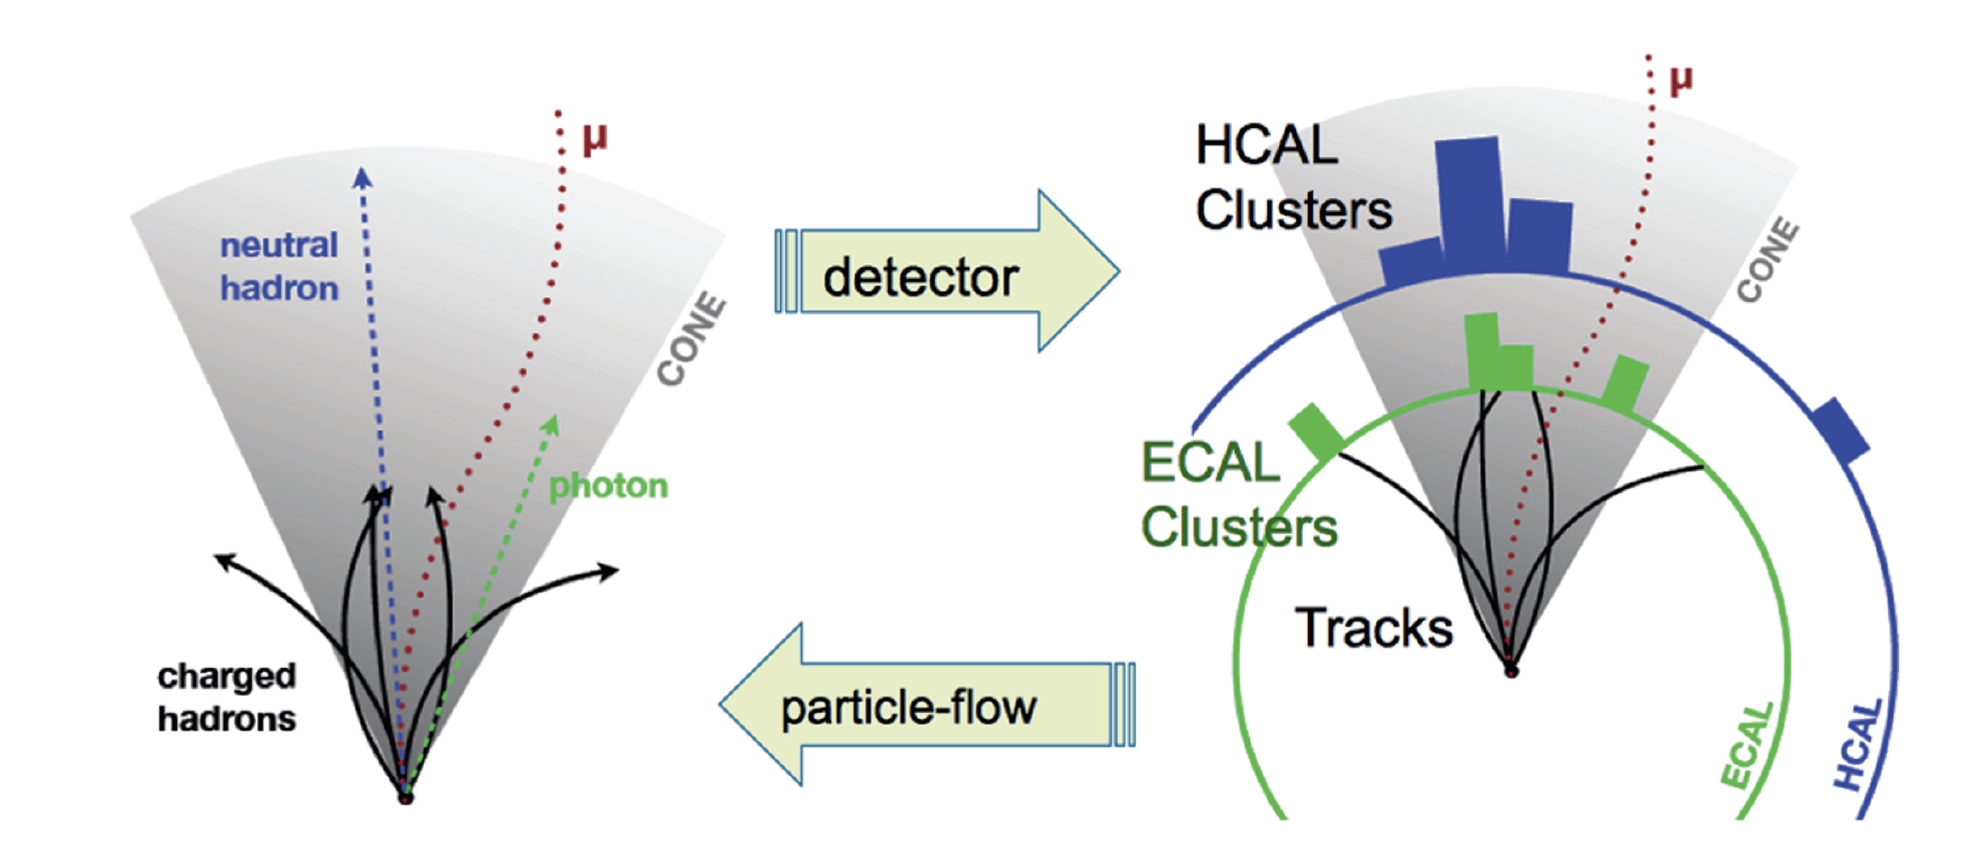
\includegraphics[width=0.58\textwidth]{Figures/c2/pfscheme}\\
\caption{The output of the PF is a list of candidates like
  electrons, muons, photons and hadrons. The PF algorithm links
  information from all the sub-system to give a global description of
  the collision event~\cite{Petrucciani:2650974}.}
\label{fig:pfscheme}
\end{figure} 

The input of the PF are the \emph{elements} tracks, vertices, tracks
reconstructed from the muon system and
calorimeter clusters. The output of the PF is a list of candidates
like electrons, muons, photons and charged and neutral hadrons (see
Figure~\ref{fig:pfscheme}). The identification of leptons, the
measurement of the \ptmiss and the categorization of the pileup tracks
are improved by the usage of the PF algorithm. When linking
information from tracker and calorimeters signals, noticeable gain is seen
in the angular momentum resolution of jets~\cite{CMS:particleflow}.

\subsubsection{Jet clustering and reconstruction}\label{sec:jetclustering}
Jets reconstruction is performed with a recombination algorithm which
is known as anti-$k_T$ algorithm (with distance parameter of cone size
of $\Delta R = 0.4$). The detailed description of the anti-$k_T$ algorithm is not
discussed in this work but all the information can be found in 
references~\cite{Cacciari_2008,Cacciari_2012}.

In order to reduce the number of jets rising from mis-reconstruction or
detector noise, identification requirements are applied depending on the single elements of the
jets meaning the number of particles and the amount of energy of the
jet which comes from different type of PF candidates~\cite{CMS-PAS-JME-16-003}.
The jet energy is set as the vectorial sum of the momenta of the
particles constituting the jet. In order to alleviate the effect of
pileup contribution in the jet reconstruction, charge hadrons
associated to pileup vertices do not enter in the jet clustering. This
scheme is known as ``charge hadron
subtraction''~\cite{CMS-PAS-JME-14-001} and removes a
considerable fraction of charged pileup particles.  
Subsequently it is applied a correction to account for the
contribution from neutral particles from pileup; the subtraction is
based on the average transverse momentum, \pt, per unit area in the
pileup jets~\cite{CACCIARI2008119, Cacciari_2008_area,
  Sirunyan:2020foa}.

Corrections on the jet energy are applied in order to correct for the
remaining pileup energy contributions and for any discrepancies
between jet properties in measured data and in simulated events. Those
correction are obtained from the ratio between the \pt of a
reconstructed jet and its corresponding generated jet and they are
measured as function of \pt and $\eta$ and applied to data and
simulation~\cite{Khachatryan_2017}. The jet \pt resolution is
derived both in data and MC and the resolution in the simulation is
fixed and smeared to match the one in the
data~\cite{Khachatryan_2017}.

\subsubsection{Tagging of jets originating from b
  quarks}\label{sec:tagging}
The identification of jets which originate from b quarks, called
b jets, can be achieved using
specific properties and features of heavy
quarks inside the jet. This technique, usually called b tagging, is
extremely important to discriminate between signal and background as
it will be analyzed and explained in Chapters~\ref{Chapter5}
and~\ref{Chapter6}.
\begin{figure}{h}
  \begin{center}
    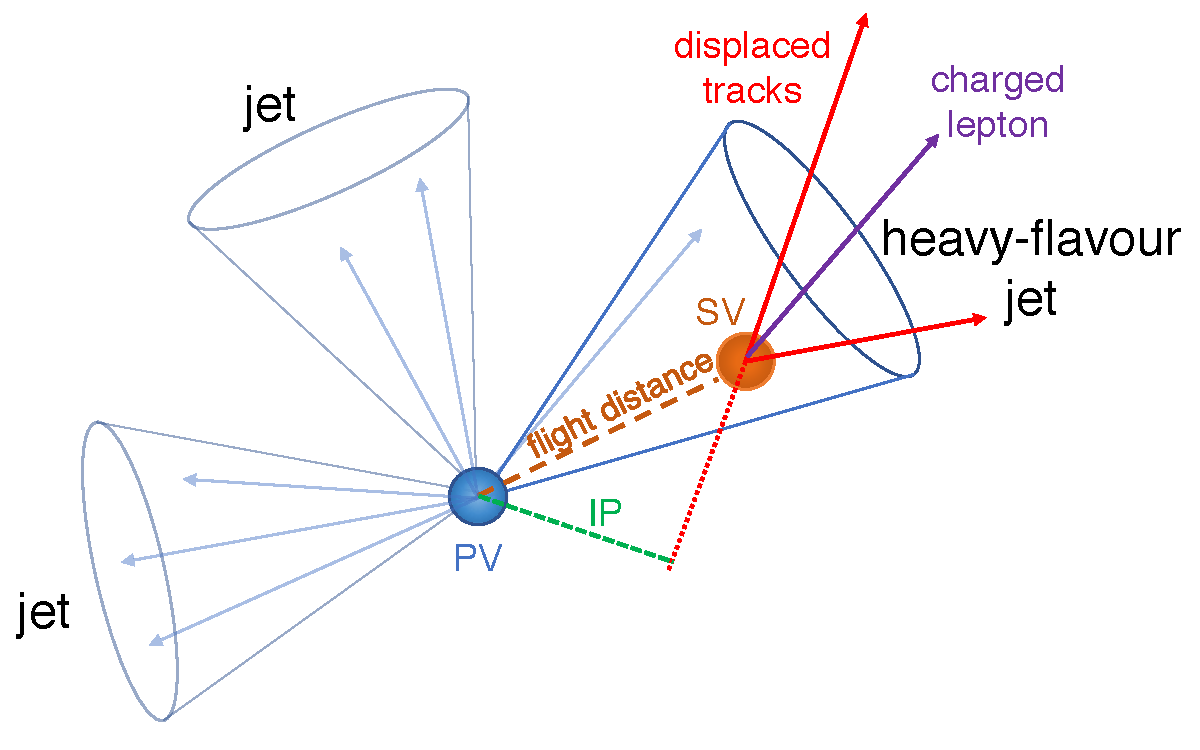
\includegraphics[clip,trim=0.3cm 0.5cm 0.3cm 0.3cm, width=0.50\textwidth]{Figures/c2/tagging}
  \end{center}
  \caption{Schematic view of a b jet with a SV from the decay of a b hadron resulting in tracks which are displaced with respect to the PV, and hence with a large impact parameter (IP) value~\cite{Sirunyan_2018_tagging}.}
\label{fig:btagging}
\end{figure}

The b jets contain b hadron that have a lifetime of the order of 1.5
ps and a mass of about
5\GeV. Thus the b hadrons can propagate from
the PV for a few mm up to a few cm before decaying. This results in
a secondary vertices (SVs) which contain displaced tracks, see
Figure~\ref{fig:btagging}. With respect to light jets (coming from
u, d, s quarks or gluons) b jets have larger mass and harder hadronization which
means that the decay products have larger momentum and larger number
of tracks related with the jet. These signatures are exploited by the
algorithms allowing to construct variables to separate b jets from
light jets. The results of the b tagging are discriminator values for
jets, see Figure~\ref{fig:taggingperformance}; large discriminator values coincide with higher probability for
the jet to be a jet originating from b hadrons~\cite{CMS-DP-2017-013,
  csv}.\\
The b tagging performances are checked in terms of the b jet
efficiency (which expresses the fraction of all b jets truly coming from b hadron
that are identified as b jets) and of misidentification probability
(which expresses the fraction of light jets or jets from c hadrons
which are identified as b jets), see
Figure~\ref{fig:taggingperformance}. 

\begin{figure}[h]
\centering
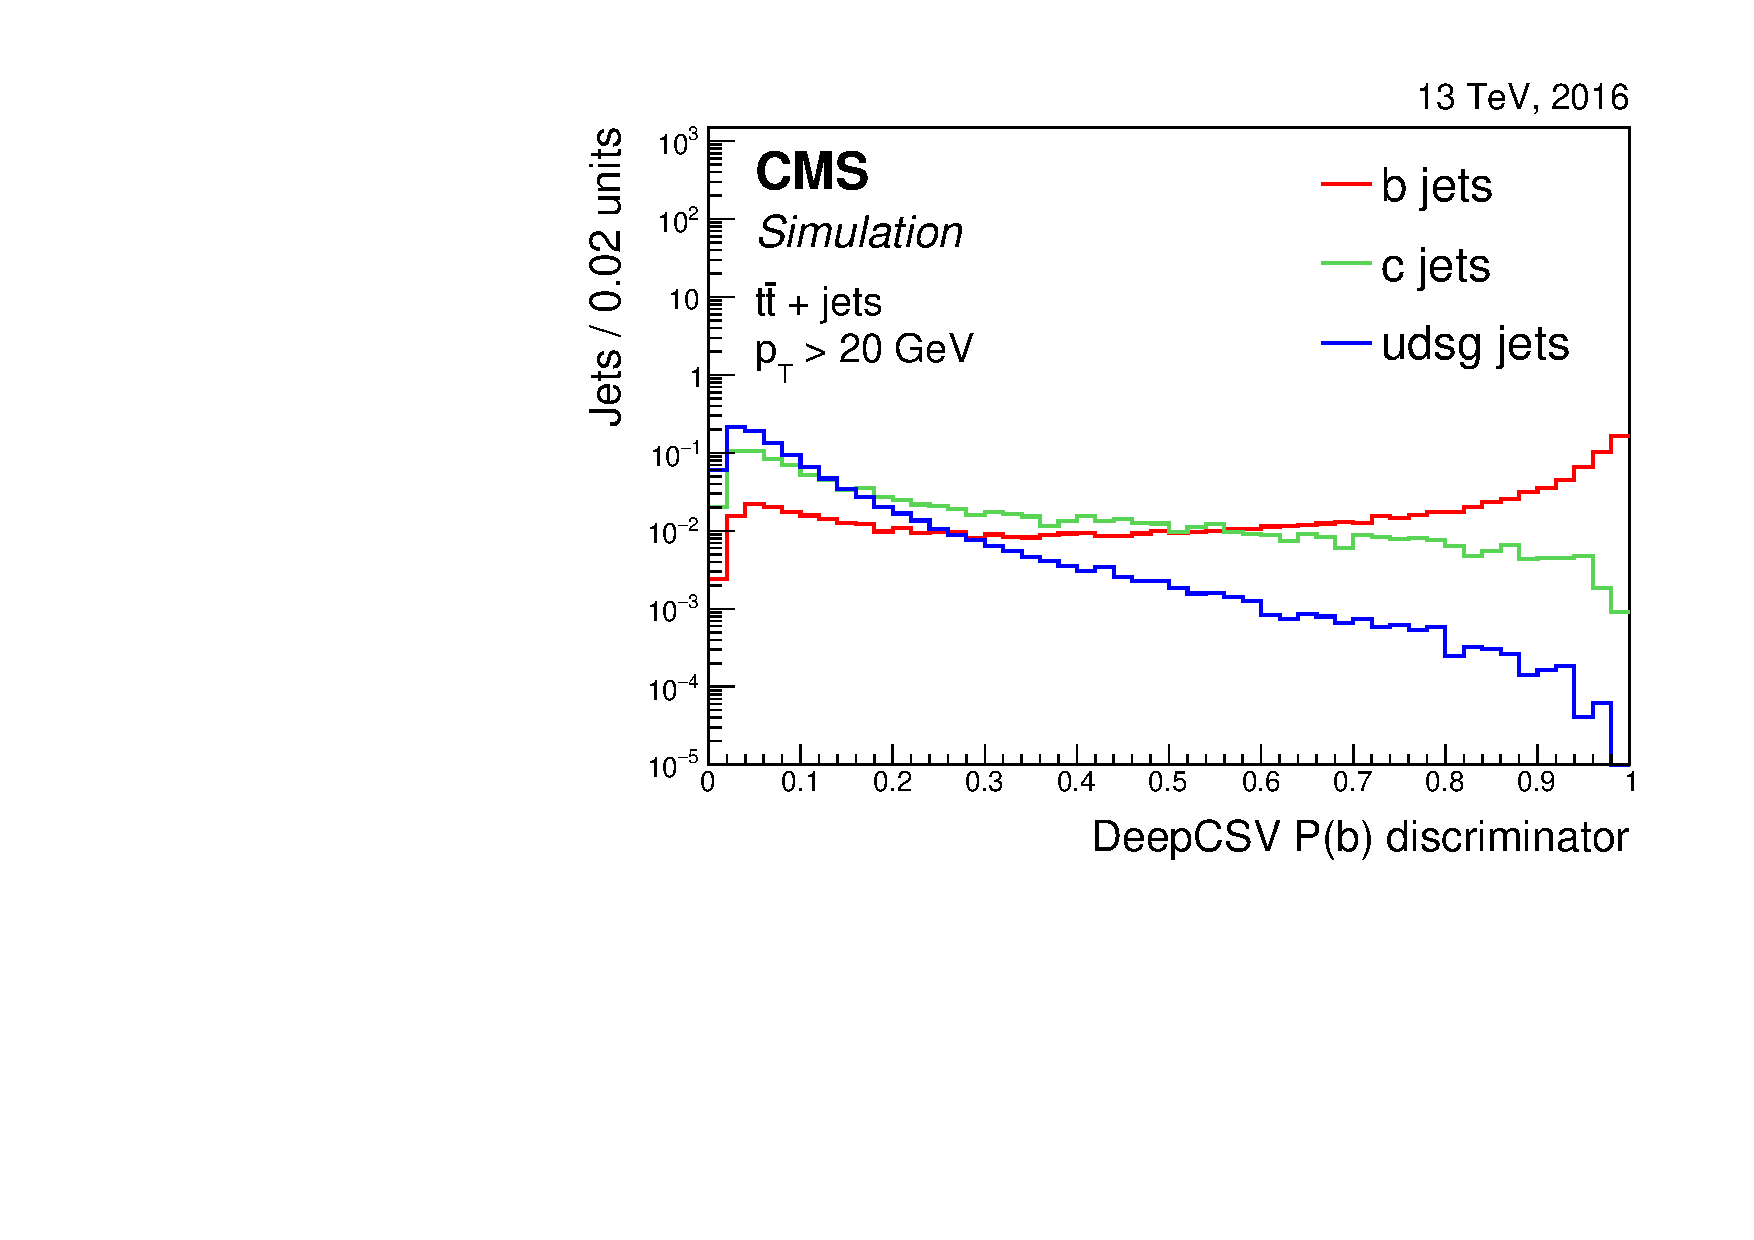
\includegraphics[width=.49\textwidth]{Figures/c2/CMS-BTV-16-002_Figure_013-a.pdf}
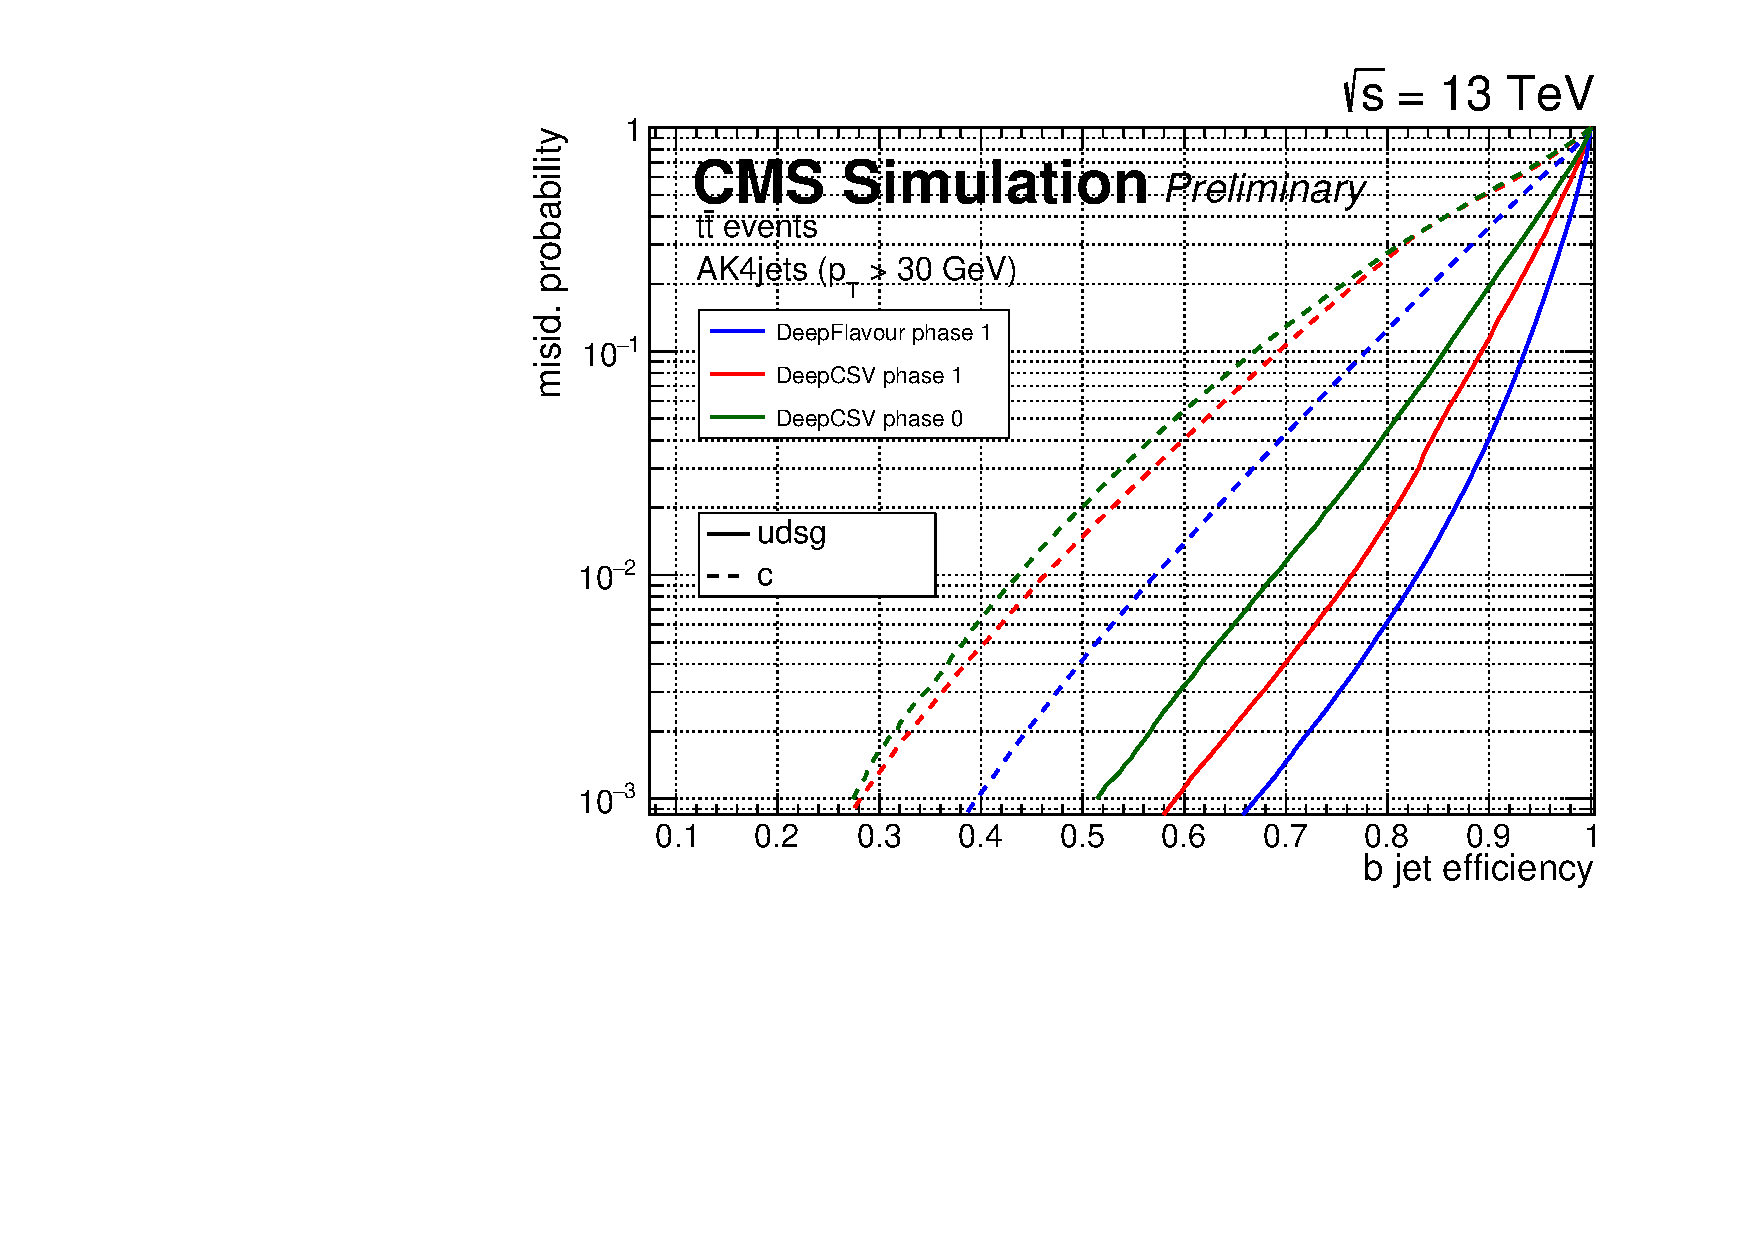
\includegraphics[width=.49\textwidth]{Figures/c2/PT30GeV.pdf}
\caption{On the left, ``performance of the DeepCSV and DeepFlavour b
  jet identification algorithms demonstrating the probability for
  non-b jets to be misidentified as b jet, as a function of the
  efficiency to correctly identify b jets. For comparison, the performance of DeepCSV
  with the 2016 detector (Phase 0) are also shown.''~\cite{csv}. On
  the right, ``Distribution of the DeepCSV P(b) discriminator values
  for jets of different flavors in \ttbar events. Jets without a
  selected track and without a secondary vertex are assigned a
  discriminator value of 0. The distributions are normalized to unit area''~\cite{csv}.}
\label{fig:taggingperformance}
\end{figure}

Here the two algorithms are known as DeepCSV~\cite{csv} and 
DeepJet~\cite{deep}. The first is the \emph{deep combined secondary vertex}, DeepCSV,
algorithm based on a fully-connected neural networks with a fixed set
of input variables for preselected tracks and preselected SVs and
kinematic features of the jets. The DeepJet~\cite{deep} is a improved
version of the DeepCSV. It is based on a deep neural network
architecture and it does not require any prior preselections and uses
a bigger number of SVs, tracks and neutral hadrons.
Looking at the right plot of Figure~\ref{fig:taggingperformance},
fixing the misidentification probability the DeepCSV has lower b jet
efficiency than DeepJet algorithm.\\
The efficiencies are calculated both in data and MC and the
corrections for the discrepancies observed between data and MC are
applied to simulated events as per-jet scale factors~\cite{csv}.


\subsection{Muon reconstruction}\label{sec:trackmuon}
This paragraph primarily describes the prompt muon reconstruction (~\ref{sec:c2muonselection}) and
identification (~\ref{sec:c2muonreco}). It will follow a short description of the displaced
case and the improved algorithms which have been designed for these specific
scenarios (~\ref{sec:c2muondisplaced},~\cite{CMS-DP-2015-015}).

\subsubsection{Muon track reconstruction}\label{sec:c2muonreco}
Muon tracking~\cite{collaboration_2013,Sirunyan_2018_muon} makes use of information from
both inner tracker and muon systems. The
inner tracker gives a precise measurement of the muon momentum; the
muon system identifies muon objects over a wide acceptance with high efficiency. A high purity in muons is obtained
thanks to the upstream ECAL and HCAL which absorb other particles
(except neutrinos). \\
According to the tracking algorithms which are used, three kinds of muon
candidates are defined~\cite{Sirunyan_2018_muon}:
\begin{itemize}
\setlength\itemsep{-0.2em}
\item \textbf{standalone muon}. The tracks are built from the
  information from all the muon sub-detectors, CSC, DT and RPC. It
  starts from seeds consisting of groups of DT or CSC segments, and
  the seeds are used for the pattern recognition in the muon system, to
gather all DT, CSC, and RPC hits along a muon trajectory using a
Kalman filter technique. The outcome of the fitting is called a
\emph{standalone-muon track}.
\item \textbf{tracker muon}. These tracks are formed
  ``inside-out''. They are extrapolated from the inner
  tracker to the muon system with loose matching to DT and CSC
  segments -- each inner track that has \pt$>0.5$\GeV and total
  momentum $>2.5$\GeV is extrapolated to the muon chambers and if at
  least one muon system segment matches that track than the muon track is defined as \emph{tracker
  muon track} --. 
\item \textbf{global muon}. These tracks are built
  ``outside-in''. They the results of the matching between
  standalone-muon tracks and tracker tracks. The matching is performed by
  comparing tracks parameters which are propagated onto a shared
  surface. Using data from both the two tracks, it is performed the final combined fit with the Kalman filter technique.
\end{itemize}

About 99\% of the muons produced within $\eta < 2.4$ are reconstructed
either as a global muon track or as a tracker muon track (or
both). In case a global muon and a tracker muon share the same inner
track, they are then merged in one single candidate.
Global muons reconstruction is meant to be very efficient for muons
which penetrate
through more than one layer of the muon system. This implicitly
requires the muon track to be more than 10\GeV since softer muons
easily fail this due to larger multiple scattering in the material of the return yoke; for the cases with
\pt$< 10$\GeV, the tracker reconstruction becomes then more efficient.
For muons which are not global muons and
they are matched with the innermost muon station only,
the probability for misidentification increases. The possibility for
hadron shower to reach the innermost muon station (punch-through)
becomes not negligible. In order to mitigate this effect additional
quality criteria on the muons are required at a later stage (described
in the following paragraph~\ref{sec:c2muonselection}).
By using the information from both the
inner tracker and the muon
system, the \pt resolution and measurement of global muons is improved
in particular for \pt $> 200$\GeV. For the case of standalone-muon
tracks, the muons have worse momentum resolution and a higher
contamination of cosmic muons than global or tracker muons.

Reconstructed muon tracks are given as input to the PF algorithm which
combines then all the information gathered from the different
sub-detectors. For muon case PF applies a list of selection criteria
to the candidates which have been reconstructed with standalone, track
and global muon algorithms. 

\subsubsection{Muon identification}\label{sec:c2muonselection}
According to the desired compromise, for each CMS search, between efficiency and purity, a
set of different variables and selections is defined~\cite{Sirunyan_2018_muon}.\\
This level of details, here described, is going to be recalled and
used in Chapter~\ref{Chapter6} where a customized and mindful selection is needed
for the displaced muon case (specifically Section~\ref{sec:c6muons}).

Some variables are related to the muon reconstruction itself. We can
list the \emph{track fit $\chi^2$}, the number of hits per track (it refers
to inner tracker hits, \emph{fraction of valid tracker hits}) and for global muons, the
level of \emph{position matching} between the tracker tracks and the standalone muon
tracks. Additionally the \emph{muon segment
compatibility} is an important parameter which returns values between 0
and 1 with 1 being the highest degree of compatibility. A \emph{kick
  finder} algorithm is deployed to evaluate a posteriori for each muon
track the
probability of being a single track or the combination of two
separated tracks.  \\
Other variables benefit from inputs from outside the muon track
reconstruction itself such as the track-PV compatibility.

Exploiting these variables, three main identification types of muons
are used in CMS physics analyses:
\begin{itemize}
\setlength\itemsep{-0.2em}
\item \emph{Loose muons identification, (Loose ID)}. A loose muon is either a
  tracker muon or a global muon. Loose ID tries to identify muons
  coming from the PV and from light and heavy flavor decay keeping
  very high selection efficiency and rather low misidentification rate
  of charged hadrons as muons. 
\item \emph{Medium muons identification, (Medium
    ID)}~\cite{PetruccianiBotta}. This selection aims to achieve, with
  respect to Loose ID, more rejection	
of muons from hadron decays in-flight while preserving
high selection efficiency. Medium muons are loose muons with tracker
tracks which have at least 80\% of valid hits in the inner tracker. 
If the muon is only a tracker muon (not a global muon), the muon
segment compatibility has to be larger than
0.451. If the muon is both a tracker muon and a global muon, ``the
muon segment compatibility need only be greater than 0.303, but then the global fit
is required to have goodness-of-fit per degree of freedom ($\chi^2$/dof) less than 3, the
position match between the tracker muon and standalone-muon must have $\chi^2$ < 12,
and the maximum c2 computed by the kink-finding algorithm must be less than 20.
The constraints on the segment compatibility were tuned after application of the
other constraints to target an overall efficiency of 99.5\% for muons from simulated
\PW and \PZ events.''~\cite{Sirunyan_2018_muon}.
\item \emph{Tight muons identification, (Tight ID)}. A tight muon must
  be reconstructed both as global muon and tracker muon. With respect
  to the Medium ID, the Tight ID requirements are more stringent on
  the number of muon stations which have to match with the inner
  tracker track and on the compatibility between track and PV. 
\end{itemize}
There are other two identification types of muons, \emph{soft muon ID}
and \emph{high momentum muon ID} which are not used in the context of
this thesis analysis and therefore are not detailed in this section. 

\paragraph{Muon isolation}\label{sec:muoniso}
To discriminate between prompt muons and muons coming from either the decays
of heavy-flavor hadrons or the decay in flight of charged $\pi^{\pm}$s and kaons, the isolation variable appears to be one of
the most critical variable to use. The PF isolation of a reconstructed
leptons is defined relative to its \pt as the scalar
sum of the energy of all the PF candidates emitted around the
direction of the muon in the cones, $\Delta R = \sqrt{(\Delta
  \phi)^2+(\Delta \eta)^2}$, surrounding the object.\\
For the estimation of the PF isolation~\cite{CMS:particleflow}, it is computed the sum of the
\pt of charge hadrons and the \pt of neutral particles (hadrons
and photons) originating from the PV. Typical values used for  $\Delta
R$ are 0.3 and 0.4.\\
A correction is applied to account for the contribution from pileup to the
neutral particles component~\cite{Sirunyan_2018_muon}.

\paragraph{Tracking and reconstruction efficiencies.}\label{sec:c2effmuon}
The efficiencies of the muon reconstruction and identification are
estimated in data and simulation events with a \emph{tag-and-probe}
method. The events are selected with two muons whose invariant mass,
$M_{\mu \mu}$, is compatible with the \PZ mass. One of the two muons,
the \emph{tag}, is selected with tight requirements. The value of the
efficiency for a specific selection (reconstruction or identification
variables) is given by the fraction of the other muons, the
\emph{probes}, which pass that specific selection. The differences in
efficiencies between data and simulation samples are accounted and
then corrected with per-muon scale factors applied to the simulated
events~\cite{Sirunyan_2018_muon}. The performances of muon
reconstruction and identification in CMS using the data collected in
2016 are shown in Figure~\ref{fig:2016eff} (details and 2017-2018
results in the reference here:~\cite{CMS-DP-2017-007,CMS-DP-2018-042})

\begin{figure}[h]
\centering
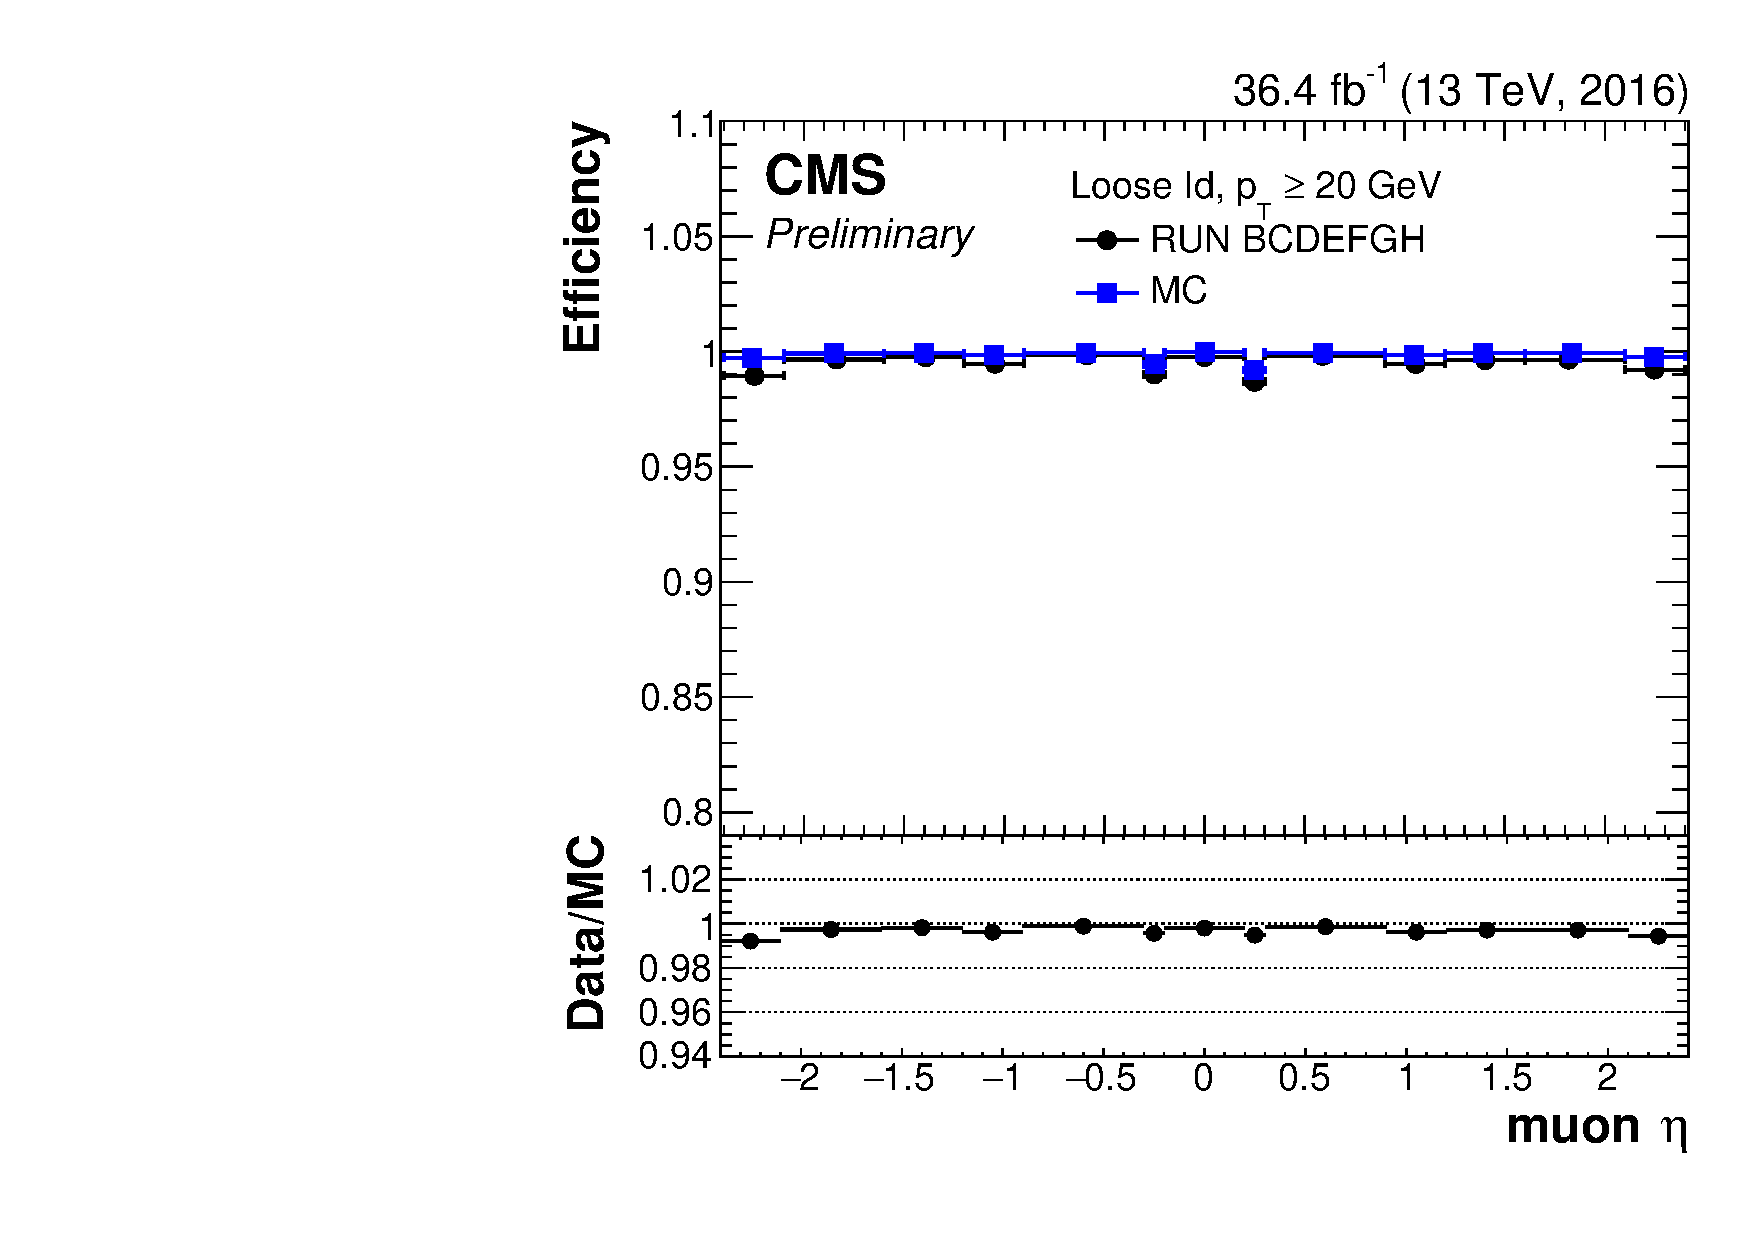
\includegraphics[width=.49\textwidth]{Figures/c2/TnP_MC_NUM_LooseID_DEN_genTracks_PAR_eta_.pdf}
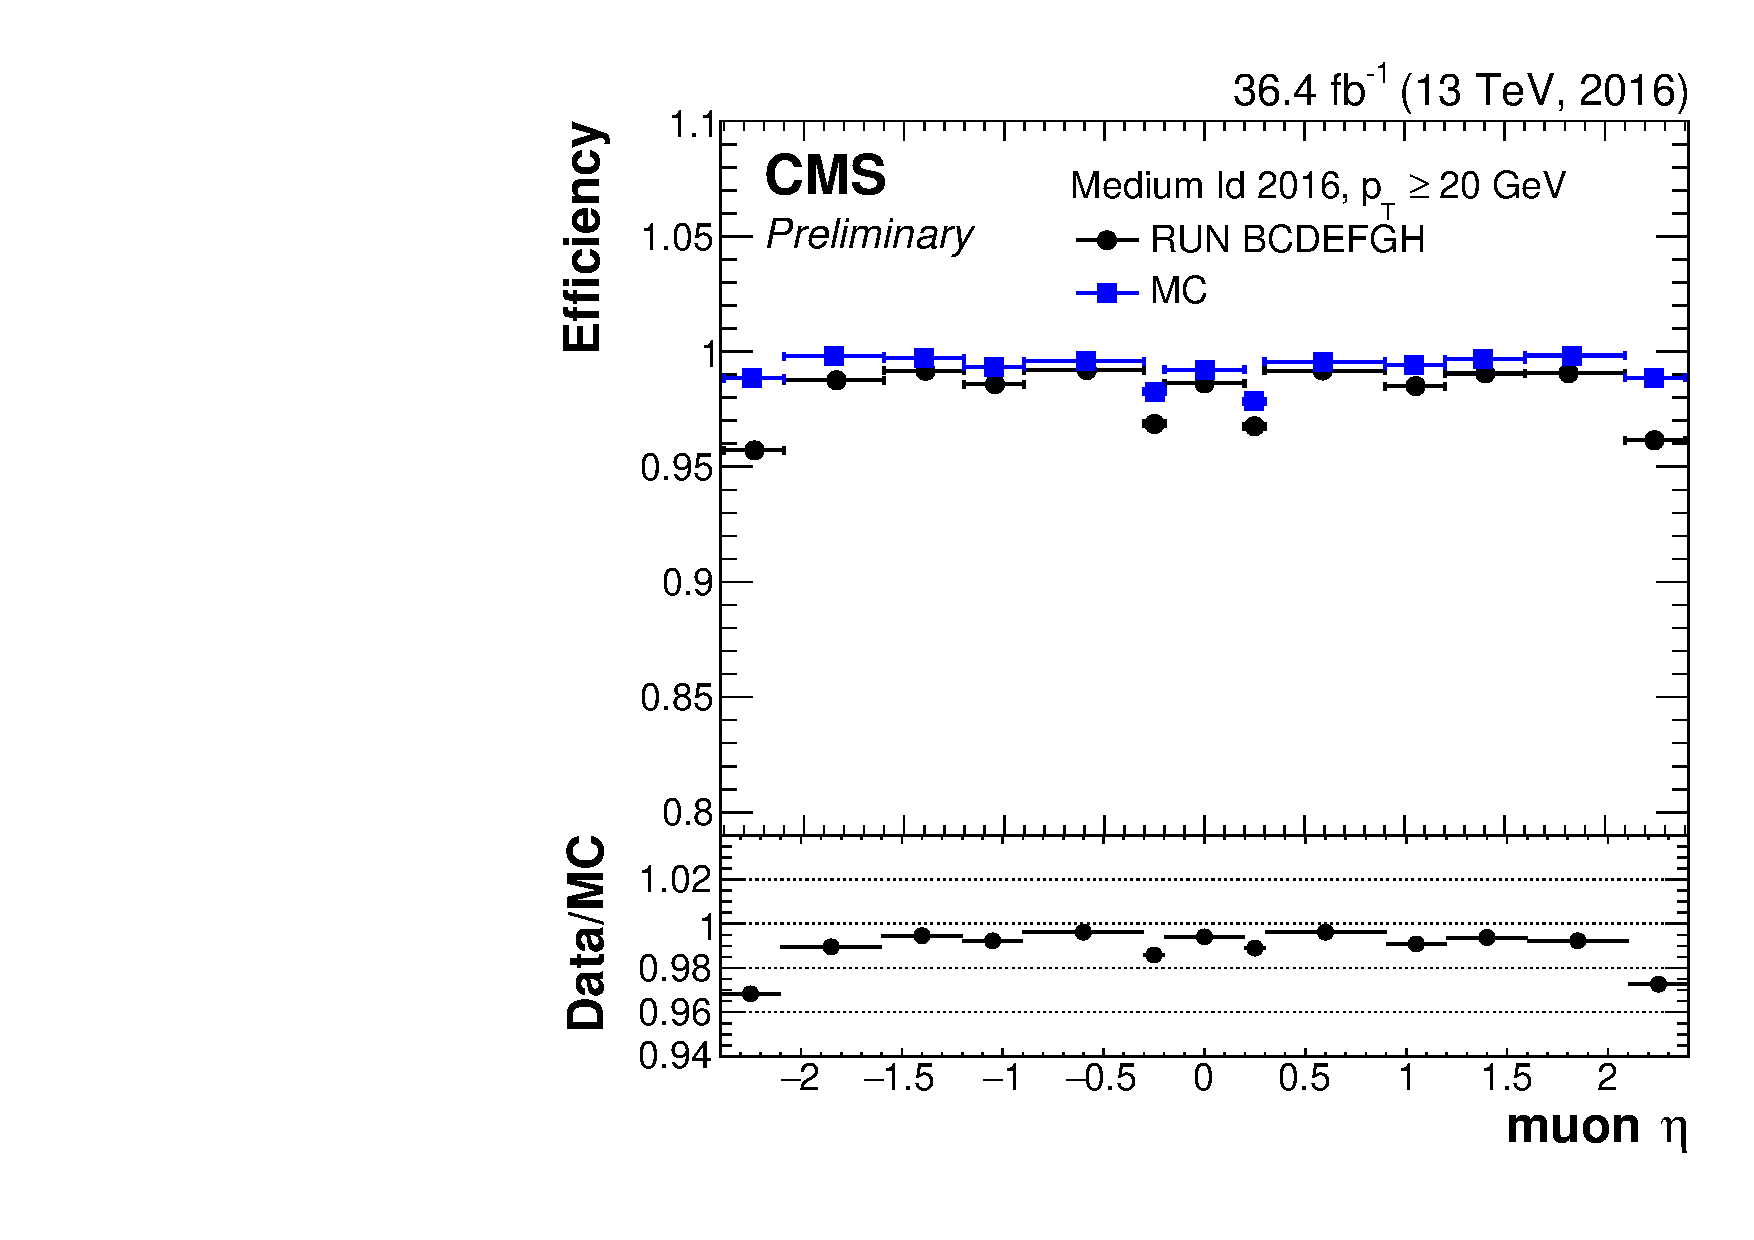
\includegraphics[width=.49\textwidth]{Figures/c2/TnP_MC_NUM_MediumID2016_DEN_genTracks_PAR_eta_.pdf}
\caption{Tag-and-probe efficiency for muon identification in 2016 data
  (circle) and simulation (squared). On the left, Loose ID efficiencies as function of $\eta$. 
On the right, Medium ID efficiencies as function of $\eta$. The
  denominator contains tracker muons. Error bars in the plots include only statistical uncertainty~\cite{CMS-DP-2017-007}}
\label{fig:2016eff}
\end{figure}


\subsubsection{Displaced muons
  reconstruction.}\label{sec:c2muondisplaced}
The search for Heavy Neutral leptons presented in
Chapter~\ref{Chapter6} includes the long-lived neutrinos scenario with
the presence  in the final
state of displaced leptons, muons and electrons,. Although CMS detector was initially designed and optimized for prompt
object reconstruction and identification, it appears to give
promising performances even for displaced object
reconstruction. Several studies and improvements on displaced muon
reconstruction have been recently
delivered, helping in the challenging effort of including long-lived
exotic searches in the CMS results (few
examples:~\cite{cmscollaboration2021search, Sirunyan_2019ll,
  Sirunyan_2019ll2, Sirunyan_2020ll, Sirunyan_2021ll,CMS:2021tkn}).

\begin{wrapfigure}{l}{0.5\textwidth}
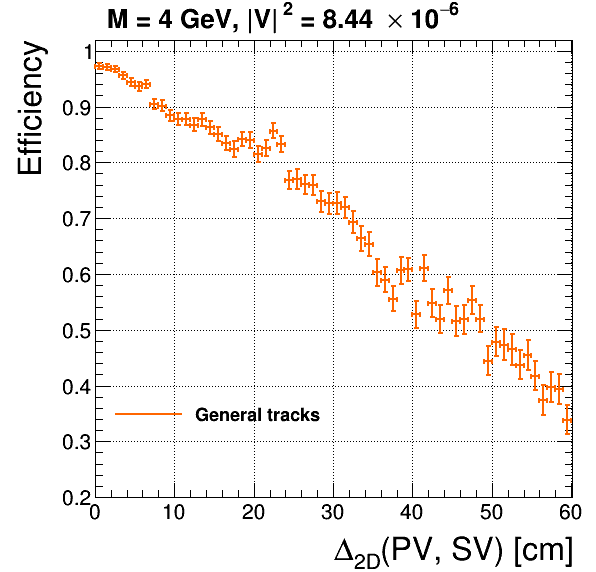
\includegraphics[width=.40\textwidth]{Figures/c6/object/tracking_M-4_V-0p00290516780927_rho.png}
  \caption{Efficiency of reconstructed inner tracker tracks with
    respect to generated muons. A HNL scenario with
    $(\mhnl,\mixparm)=(4\GeV,8.44\times10^{-6})$ is used as
    benchmark. \dani}
  \label{fig:c2tracking}
\end{wrapfigure}
The analysis presented in Chapter~\ref{Chapter6} makes use of the
standard reconstruction which
 is explained in
Section~\ref{sec:c2muonreco}. 
Fig.~\ref{fig:c2tracking} shows the efficiency of
reconstructing a muon track in the inner tracker. The efficiency is
calculated as pure reconstruction efficiency with respect to the
generated tracks. The variable which is used to display the reconstruction
performance is the 2D distance between the PV and the secondary vertex
which is one of the best proxies to estimate the point of orgin of the
displaced muon. The efficiency worsens when trying to reconstruct
muons which have created towards the external layers of the inner
tracker. Figure.~\ref{fig:c2tracking2} shows, on the left, the sequential
efficiencies of the plain PF Muon requirement, Loose ID, and
valid tracker hit fraction requirement (refer to Section~\ref{sec:c2muonselection}), with respect to the reconstructed
inner-tracker track. It is clear that the efficiency of
this last selection falls rapidly with increasing of the PV-SV
distance. 

\begin{figure}[h]
\centering
  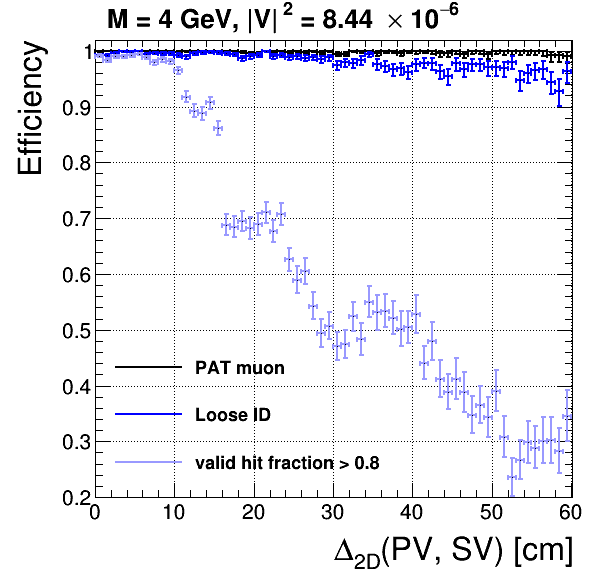
\includegraphics[width=0.40\textwidth]{Figures/c6/object/loose_validFraction_M-4_V-0p00290516780927_rho.png}
  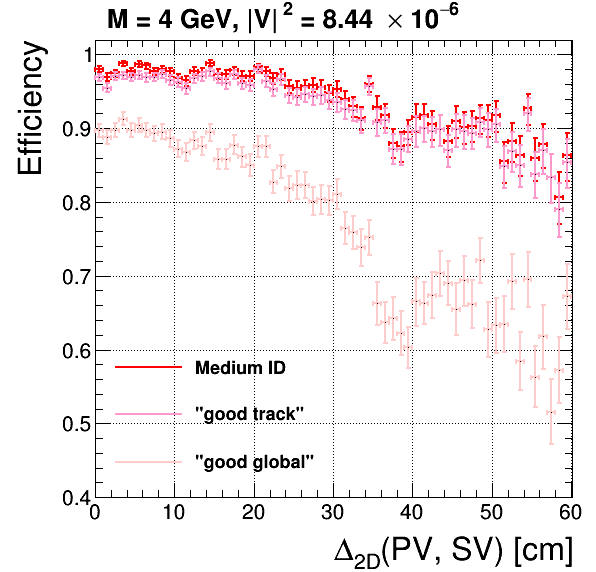
\includegraphics[width=0.40\textwidth]{Figures/c6/object/goodTrack_goodGlobal_M-4_V-0p00290516780927_rho.png}
  \caption{On the left, the sequential
efficiencies of the plain PF Muon requirement, Loose ID, and
valid tracker hit fraction requirement is shown. On the right, the efficiency of the tracker-muon only and
    global-muon only requirements is compared with their logical OR
    efficiency (using already the custumized Medium ID). A HNL scenario with
    $(\mhnl,\mixparm)=(4\GeV,8.44\times10^{-6})$ is used as
    benchmark. \dani}
  \label{fig:c2tracking2}
\end{figure}

The valid-hit fraction request is thus removed from the set of
requirements of the Medium ID (refer to Section~\ref{sec:c2muonselection}), and is not applied in the following
efficiencies. To mitigate the depreciation of the
total efficiency for muons not emerging from the primary vertex, the
Medium ID is then modified in the context of the analysis presented in
Chapter~\ref{Chapter6}.
\begin{wrapfigure}{r}{0.5\textwidth}
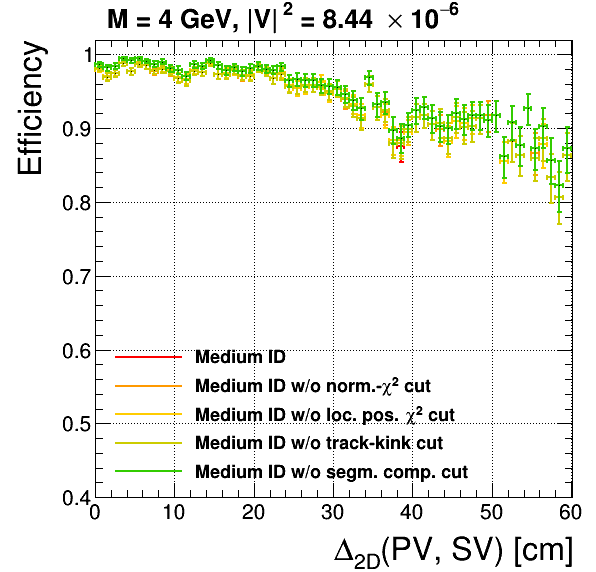
\includegraphics[width=.40\textwidth]{Figures/c6/object/globalTrack_cuts_M-4_V-0p00290516780927_rho.png}
  \caption{Efficiency of different Medium-ID selections with respect to tracks for displaced
muons. A HNL scenario with
    $(\mhnl,\mixparm)=(4\GeV,8.44\times10^{-6})$ is used as
    benchmark. \dani}
  \label{fig:c2tracking3}
\end{wrapfigure}
In Figure.~\ref{fig:c2tracking2}, on the
right, it is shown the comparison between the efficiencies of the
tracker-muon only and global-muon only and their logical OR (\ie, the full
modified Medium ID). The main contribution to the efficiency comes
from the tracker-muon selection, while the addition of the global-muon
selection only increases the overall efficiency by few percent.\\
Finally, Fig.~\ref{fig:c2tracking3} compares the efficiency of
the full custumized Medium ID with the efficiencies obtained by removing
individual requirements from the global-muon definition. None of these variables
appears to hurt the overall efficiency significantly---the larger
effect is observed for the segment-compatibility cut of 0.303, and it
amounts to 1--2\%. Additionally, none of the cuts on the global-track
variables depends on the displacement.









~\cite{CMS-DP-2015-015}
\clearpage
\subsection{Tracking for electrons}\label{sec:trackele}



\paragraph{Muon and electron Isolation}\label{sec:muoniso}
To discriminate between prompt leptons and leptons coming from either the decays
of heavy-flavor hadrons or the decay in flight of charged $\pi^{\pm}$s and kaons, the isolation variable appears to be one of
the most critical variable to use. The PF isolation of a reconstructed
leptons is defined relative to its \pt as the scalar
sum of the energy of all the PF candidates emitted around the
direction of the lepton in the cones, $\Delta R = \sqrt{(\Delta
  \phi)^2+(\Delta \eta)^2}$, surrounding the object.\\
For the estimation of the PF isolation~\cite{CMS:particleflow}, it is computed the sum of the
\pt of charge hadrons and the \pt of neutral particles (hadrons
and photons) originating from the PV. Typical values used for  $\Delta
R$ are 0.3 and 0.4.\\
A correction is applied to account for the contribution from pileup to the
neutral particles component~\cite{Sirunyan_2018_muon}.



~\cite{CMS:particleflow}
~\cite{Collaboration_2014_tracking}
~\cite{Collaboration_2010_alligment}


Figure 16 shows the invariant mass distribution of oppositely charged muon pairs selected by
the inclusive trigger on isolated double-muons. The x-axis is logarithmic so the entries are
scaled to the width of each bin. Data are also included from specific double-muon triggers
tuned to select resonances at low invariant mass. The figure clearly demonstrates the ability of
CMS to identify muons, trigger on them, and reconstruct the muon kinematics to unambiguously
identify particles that decay into muons over a broad energy range.
 \begin{figure}[h]
\centering
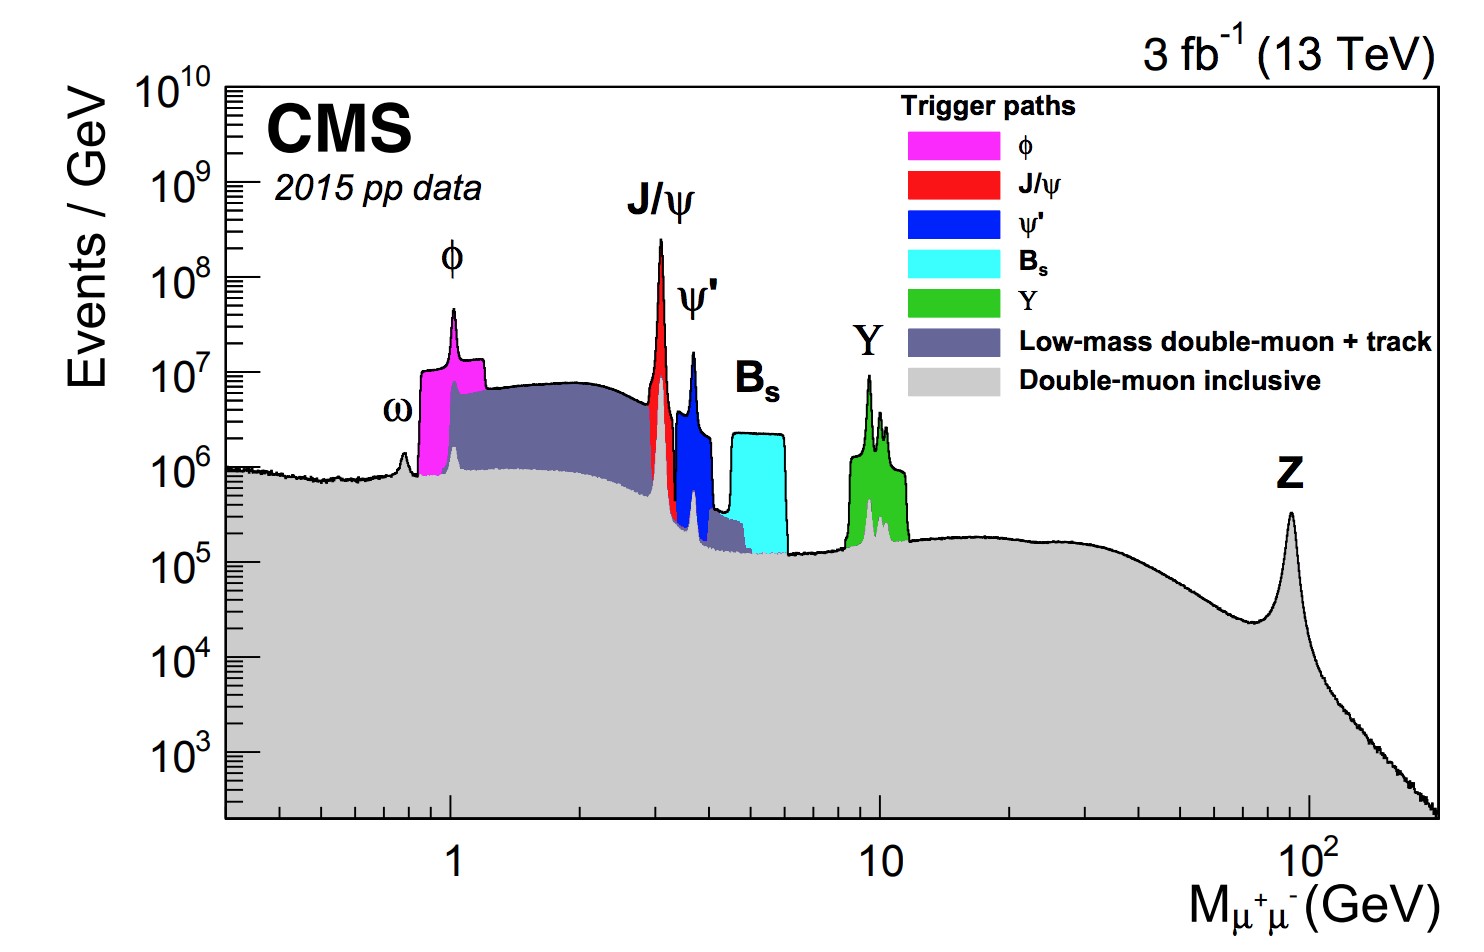
\includegraphics[width=.88\textwidth]{Figures/c2/dimuon}
\caption{``The dimuon invariant mass distribution reconstructed by the CMS HLT. Data were
collected in 2015 with the inclusive double-muon trigger algorithm (gray), as well as triggers
dedicated to selecting resonances at low masses.''~\cite{Sirunyan_2018_muon}.}
\label{fig:dimuon}
\end{figure}






\subsection{Track reconstruction} 
Electron reconstruction is based on the combination of tracker and
ECAL information in a Gaussian Sum Filter (GSF)
track~\cite{Khachatryan:2015hwa}, which accounts for possible
bremsstrahlung from the electron.
Electrons are reconstructed within the geometrical acceptance of the
CMS tracking system, $|\eta|<2.5$.
Identification criteria based on the electromagnetic shower shape, track
quality, track impact parameters with respect to the primary vertex,
and isolation are used to select signal electrons and reduce the rate
of mis-identified and background electrons (referred to as ``fake
electrons'' hereafter).

Muons are reconstructed by combining the information of the tracker
and of the muon
spectrometer~\cite{Sirunyan:2018fpa}.
The geometric compatibility between these separate measurements is
used in the further selection of muons. Muons are required to have
$\abseta<2.4$ to fall inside the geometric acceptance of the muon
detector.
All muons considered for analysis must pass the loose working point as
specified by the MUO POG, in addition to a number
of other loose criteria on isolation and their impact parameters with
respect to the PV.
It is also possible to require muons to be synchronized with the bunch
crossing that has triggered, using the time measurements provided by
the muon sub-detectors, the RPCs (``RPC time'' or $t_{\mathrm{RPC}}$)
and the combined measurements of the DTs and CSCs (``combined time''
or $t_{\mathrm{comb}}$)~\cite{muon_oot}.
In particular, $t_{\mathrm{RPC}}$ ($t_{\mathrm{comb}}$) is only used
if it is measured with more than 1 (7) degrees of freedom.
If $t_{\mathrm{RPC}}$ and $t_{\mathrm{comb}}$ are both available,
they must lie within $-10\ns$ and $+10\ns$.
If only $t_{\mathrm{comb}}$ is available, then it must be within
$-45\ns$ and $+20\ns$.
If $t_{\mathrm{comb}}$ is unavailable, no timing requirement is
applied.

\subsection{Reconstruction performances}
\clearpage
